\documentclass[lettersize,journal]{IEEEtran}

% -------- Caption formatting from IEEEtran Template --------


% -------- Packages --------
\usepackage{amsmath,amsfonts}
\usepackage{array}
\usepackage[caption=false,font=normalsize,labelfont=sf,textfont=sf]{subfig}
\usepackage{textcomp}
\usepackage{stfloats}
\usepackage{url}
\usepackage{verbatim}
\usepackage{graphicx}
\usepackage{cite}
\usepackage{afterpage}
\usepackage[T1]{fontenc}
\usepackage{longtable}
\usepackage{booktabs}
\usepackage[english]{babel}
\addto\captionsenglish{\renewcommand{\figurename}{Fig.}}
\usepackage{xcolor}
\usepackage{tikz}
\usetikzlibrary{arrows.meta,positioning}
\usepackage[hidelinks]{hyperref}
\usepackage{makecell}
\usepackage{mathtools}
\usepackage{tabularx}
\usepackage{xstring} % for character count

% -------- Revision marking --------
% All text added or changed in this revision is wrapped in \rev{...} and
% printed in blue. Remove the colour (set to black) for the clean final copy.
\newcommand{\rev}[1]{#1}

% -------- Settings --------
\setlength{\jot}{2pt}
\allowdisplaybreaks[1]
\hyphenation{op-tical net-works semi-conduc-tor IEEE-Xplore}

% -------- Highlights helpers (exports to highlights.txt) --------
\newwrite\highlightsfile
\immediate\openout\highlightsfile=highlights.txt
\AtEndDocument{\immediate\closeout\highlightsfile}

\newcommand{\HighlightItem}[1]{%
  % length check (≤85 chars, incl. spaces)
  \StrLen{#1}[\hllen]%
  \ifnum\hllen>85
    \typeout{HL WARNING: item exceeds 85 chars (\the\hllen): #1}%
  \fi
  \item #1%
  \immediate\write\highlightsfile{- #1}%
}

\begin{document}

% -------- Title/Author --------
\title{Characterisation and Quantification of Data Centre Flexibility for Power System Support}

\author{ James Day\textsuperscript{1}, Mehmet Turker Takci\textsuperscript{1}, and Meysam Qadrdan\textsuperscript{1}}

% Affiliations + Highlights directly under the title
\IEEEaftertitletext{%
  \vspace{-0.5em}%
  \noindent\small
  \textsuperscript{1}Cardiff University, Queen's Buildings, The Parade, Cardiff CF24 3AA, United Kingdom\par
  \vspace{0.6em}
  % ---- Highlights (3–5 bullets, ≤85 chars each). Also written to highlights.txt ----
  \noindent\small\textbf{Highlights}\par
  \vspace{0.25em}\noindent\hrule height 0.5pt \vspace{0.35em}
  \begin{itemize}
    \setlength{\itemsep}{0.2em}\setlength{\parskip}{0pt}\setlength{\parsep}{0pt}
    % Replace the five lines below with your final 3–5 bullets (≤85 chars each)
    \HighlightItem{Integrated IT/UPS/cooling model developed for a data centre.}
    \HighlightItem{\rev{Cost-optimised operation cuts annual electricity costs by 5.05\%.}}
    \HighlightItem{Flexibility characterised and quantified by a duration-aware flexibility assessment.}
    \HighlightItem{\rev{100 kW of upward flexibility sustained for six hours by a 1 MW IT-rated DC.}}
    \HighlightItem{\rev{Additional UPS capacity is assessed using annual savings and investment thresholds.}}
  \end{itemize}
  \vspace{0.35em}\noindent\hrule height 0.5pt \vspace{0.6em}
  %
  % ---- Corresponding Author (NEWLY ADDED) ----
  \noindent\small\textbf{Corresponding author:}\par
  \vspace{0.1em} % Small space
  \noindent\small
  James Day\par
  \textit{E-mail address:} \texttt{DayJa1@cardiff.ac.uk}\par
  \vspace{0.6em} % Match spacing of other blocks
  % ------------------------------------------
}

\maketitle

% The paper headers
\markboth{Data Centre Flexibility}%
{Takci \MakeLowercase{\textit{et al.}}: Characterisation and Quantification of Data Centre Flexibility}

% -------- Abstract & Keywords --------
\begin{abstract}
The rapid growth of data centres poses an evolving challenge for power systems striving toward high variable renewable energy resources and new demands. Traditionally operated as passive electrical loads, data centres, as large loads now, have the potential to become active participants that provide flexibility to the grid. However, quantifying and utilising this flexibility have not yet been fully explored. This paper presents an integrated, whole facility optimisation model to investigate the least cost operating schedule of data centres and characterise the aggregate flexibility available from data centres to the power system. The model accounts for IT workload shifting, UPS energy storage, and cooling system. Motivated by the need to alleviate the increasing strain on power systems while leveraging their untapped flexibility potential to support decarbonisation goals, this study makes two primary contributions: (i) an operational optimisation model that integrates IT scheduling, UPS operation, and cooling dynamics to establish a cost optimal baseline operation, and (ii) a duration-aware flexibility assessment that, for any given start time and requested power deviation, identifies a certified feasible duration from this baseline while respecting all operational, thermal, and recovery constraints. \rev{This second contribution is the main grid-facing advance of the paper: it converts a data centre's latent flexibility into a time-certified envelope of feasible magnitude--duration offers.} Results reveal a clear temporal structure and a notable asymmetry in flexibility provision: upward flexibility (electricity load reduction) is driven by deferring IT workload, which allows for a secondary reduction in cooling power. In contrast, downward flexibility (electricity load increase) combines changes in IT execution, cooling and storage; eligible work can execute earlier than in the baseline, but never before arrival. \rev{For the 1 MW IT-rated case study, 100 kW of upward flexibility can be sustained for six hours at noon and 1.25 hours at 06:00, demonstrating the strong dependence of feasible duration on the baseline operating state. Linked daily optimisation over 2025 gives a 5.05\% annual electricity-cost saving; resource sensitivities examine workload share, UPS and TES capacity.} This framework translates abstract flexibility potential into quantified flexibility magnitude and duration capability that system operators could investigate for use in services such as reserve, frequency response, and price responsive demand.
\end{abstract}

\begin{IEEEkeywords}
Data Centre, Power system flexibility, Demand side flexibility, Load Shifting, Thermal Inertia
\end{IEEEkeywords}
% --- NO \onecolumn HERE ---

% --- START YOUR PAPER'S BODY TEXT (e.g., INTRODUCTION) ---
\section{Introduction}

\IEEEPARstart{G}{lobal} digitalisation, propelled by artificial intelligence, is driving the rapid expansion of data centres, whose electricity demand is both substantial and spatially concentrated. This growth coincides with two other major shifts in the energy landscape: the increasing share of variable renewable generation needed for decarbonisation, and the widespread adoption of new demand-side technologies such as electric vehicles and heat pumps \cite{Centrica2020LEM, EEAACER2023Flex}. The combined effect places significant strain on modern power systems by intensifying peak loads, steepening net load ramps, and aggravating local network constraints. Consequently, there is an escalating need for power system flexibility to maintain the crucial balance between electricity supply and demand.

According to the IEA, global data centre electricity consumption was around 415 TWh in 2024, with projections suggesting this will exceed 945 TWh by 2030, raising their share of global electricity demand from approximately 1.5\% to 3\% \cite{iea_energy_ai}. This expansion is not uniform, with over 80\% of the increase expected to originate from the United States and China \cite{iea_energy_ai}. Moreover, geographical clustering intensifies the impact on local grids. For instance, data centre consumption already accounts for over 20\% of national demand in Ireland, and 25\% in Virginia, USA \cite{iea_energy_ai}. In Great Britain, annual electricity consumption by data centres is forecast by National Grid ESO to rise from 7.6 TWh in 2024 to between 30–71 TWh by 2050 \cite{neso2025future}.




% This text will correctly appear in TWO COLUMNS.
% --- PLACE THE \afterpage BLOCK *AFTER* THE FIRST PARAGRAPH ---
\afterpage{
\clearpage % Start a new page
\onecolumn % Switch to one column *for this page
%\section*{Nomenclature}
{\small
\renewcommand{\arraystretch}{1.15}
\begin{longtable}{p{0.1\textwidth} p{0.66\textwidth} p{0.12\textwidth} p{0.06\textwidth}}
\caption{Nomenclature} \label{tb:nomenclature} \\
\toprule
\textbf{Symbol} & \textbf{Definition} & \textbf{Value/Bounds} & \textbf{Unit} \\
\midrule
\endfirsthead
\multicolumn{4}{c}%
{{\bfseries \tablename\ \thetable{} -- continued from previous page}} \\
\toprule
\textbf{Symbol} & \textbf{Definition} & \textbf{Value/Bounds} & \textbf{Unit} \\
\midrule
\endhead
\midrule
\multicolumn{4}{r}{{Continued on next page}} \\
\endfoot
\bottomrule
\endlastfoot
% IT Workload Section
\midrule
\multicolumn{4}{l}{\textbf{IT Workload Modelling (Section 3.1)}} \\
\midrule
$t, s$ & Time slot an IT job originates in ($t$) and time slot the job is executed in ($s$). & Absolute slot indices & - \\
$T$ & Committed time slots of local day $d$; $T_d$ below. & 92, 96 or 100 slots & - \\
$T^{\mathrm{ext}}$ & Local-day core plus twelve look-ahead slots; $T_d^{\mathrm{ext}}$ below. & $|T_d|+12$ slots & - \\
$k$ & Index for tranches of a flexible IT job. & [1,2,3,4] & - \\
$K$ & Set of tranche indices, with each tranche representing a distinct deferral class. Original classes retained in Section \ref{sec:scenario 3}. & $\{1, 2, 3, 4\}$ & - \\
$W_{t,k}$ & Feasible execution window of time slots for tranche k of a job originating at time t. & Varies & - \\
$\Delta t$ & Duration of a single time slot. & 0.25 & hours \\
$D_k$ & Maximum deferral duration (in time slots) for tranche k of a job, relative to its arrival time. Original classes retained in Section \ref{sec:scenario 3}. & $\{2, 4, 8, 12\}$ & slots \\
$P^{\mathrm{IT}}_{\mathrm{idle}}$ & Power consumption of IT equipment at idle CPU utilisation. & 166.7 &kW \\
$P^{\mathrm{IT}}_{\mathrm{max}}$ & Power consumption of IT equipment at maximum CPU utilisation. & 1000 &kW \\
$u_{\max}$ & Maximum available CPU capacity in any single time slot. & 1 & - \\
$u_t^{\mathrm{inflex}}$ & CPU utilisation required for the inflexible workload in time slot t. & [0–1] & - \\
$u_t^{\mathrm{flex,base}}$ & Base CPU utilisation required to process the flexible job originating at slot t without any deferral. & [0–1] & - \\
$R_t$ & Total computational demand (in CPU-hours) for the flexible job originating in time slot t. & Varies & CPU-hours \\
$\alpha_{t,k}$ & Fraction of the total computational demand $R_t$ that is assigned to tranche k. & [0–1] & - \\
$u(t)$ & CPU utilisation at time t, as a fraction of total capacity. & [0–1] & - \\
$u(t,k,s)$ & Decision variable for the CPU utilisation of tranche k from a job originating at t, scheduled for execution in slot s. & $\geq 0$ & - \\
$P^{\mathrm{IT}}(t)$ & Total power consumption of IT equipment at time t. & [0-1000] &kW \\
$E^{\mathrm{IT}}_{\mathrm{base}}(t)$ & Base IT energy consumption at time t. & Varies &kWh \\
$E^{\mathrm{IT}}_{\mathrm{opt}}(t)$ & Optimised IT energy consumption at time t after optimisation. & Varies &kWh \\
$P^{\mathrm{IT}}_{\mathrm{base}}(t)$ & Base IT power consumption at time t. & [0-1000] &kW \\
$P^{\mathrm{IT}}_{\mathrm{opt}}(t)$ & Optimised IT power consumption at time t after optimisation. & [0-1000] &kW \\
% UPS-ESS Section
\midrule
\multicolumn{4}{l}{\textbf{UPS-ESS Modelling (Section 3.2)}} \\
\midrule
$E^{\mathrm{UPS}}_{\mathrm{base}}$ & Base rated energy capacity of the UPS battery system. & 600 &kWh \\
$SoC_{\min}$ & Minimum state of charge, expressed as a fraction of $E_{\mathrm{UPS}}^{\mathrm{base}}$. & 0.5 & - \\
$SoC_{\max}$ & Maximum state of charge, expressed as a fraction of $E_{\mathrm{UPS}}^{\mathrm{base}}$. & 1.0 & - \\
$P^{\mathrm{UPS}}_{\mathrm{ch,min}}$ & Minimum allowable charging power of the UPS. & 0 &kW \\
$P^{\mathrm{UPS}}_{\mathrm{ch,max}}$ & Maximum allowable charging power of the UPS. & 270 &kW \\
$P^{\mathrm{UPS}}_{\mathrm{disch,min}}$ & Minimum allowable discharging power of the UPS. & 0 &kW \\
$P^{\mathrm{UPS}}_{\mathrm{disch,max}}$ & Nominal UPS discharge rating; useful discharge also cannot exceed IT demand (at most 1000 kW). & 2700 &kW \\
$\eta^{\mathrm{UPS}}_{\mathrm{ch}}$ & Charging efficiency of the UPS battery system. & 0.82 & - \\
$\eta^{\mathrm{UPS}}_{\mathrm{disch}}$ & Discharging efficiency of the UPS battery system. & 0.92 & - \\
$E^{\mathrm{UPS}}(t)$ & Energy stored in the UPS battery system at the opening boundary of time slot t. & $[300, 600]$ &kWh \\
$P^{\mathrm{UPS}}_{\mathrm{ch}}(t)$ & Charging power drawn by the UPS from the grid during time slot t. & $\geq 0$ &kW \\
$P^{\mathrm{UPS}}_{\mathrm{disch}}(t)$ & Discharging power supplied by the UPS during time slot t. & $\geq 0$ &kW \\
$P^{\mathrm{UPS}}_{\mathrm{net}}(t)$ & Net power exchange of the UPS at time t, defined as $P^{\mathrm{UPS}}_{\mathrm{ch}}(t) - P^{\mathrm{UPS}}_{\mathrm{disch}}(t)$. & Varies &kW \\
$z^{\mathrm{UPS}}_{\mathrm{ch}}(t)$ & Binary variable indicating charging status in time slot t. & $\{0, 1\}$ & - \\
$z^{\mathrm{UPS}}_{\mathrm{disch}}(t)$ & Binary variable indicating discharging status in time slot t. & $\{0, 1\}$ & - \\
% Cooling System Section
\midrule
\multicolumn{4}{l}{\textbf{Cooling System Modelling (Section 3.3)}} \\
\midrule
$\dot{m}_a$ & Constant mass flow rate of air circulated by the cooling unit. & 100 & kg/s \\
$c_{pa}$ & Specific heat capacity of air at constant pressure. & 1.005 & kJ/(kg$\cdot$K) \\
$\rho_a$ & Density of air. & 1.16 & kg/m$^3$ \\
$C_{IT}$ & Total heat capacity of the IT components. & $1.788 \times 10^4$ & kJ/K \\
$C_R$ & Total heat capacity of the server racks and the air within them. & $1.802 \times 10^4$ & kJ/K \\
$C_{CA}$ & Total heat capacity of the air in the cold aisle. & $2.33 \times 10^3$ & kJ/K \\
$C_{HA}$ & Total heat capacity of the air in the hot aisle. & $1.17 \times 10^3$ & kJ/K \\
$G_{cv}$ & Convective heat conductance coefficient between IT components and rack air. & 109 &kW/K \\
$G_{cd}$ & Total heat transfer coefficient from the cold aisle to the outside environment. & 4.484 &kW/K \\
$\kappa$ & Correction factor for the effectiveness of the air mass flow through racks. & 0.766 & - \\
$COP_{\mathrm{chiller}}$ & Coefficient of Performance of the chiller. & 5 & - \\
$P^{\mathrm{Chiller}}_{\mathrm{max}}$ & Maximum electrical power consumption capacity of the chiller. & 400 &kW \\
$E^{\mathrm{TES}}_{\mathrm{max}}$ & Maximum cooling energy storage capacity of the TES tank. & 1000 &kWh \\
$Q^{\mathrm{TES}\text{-}\mathrm{CRAC}}_{\mathrm{max}}$ & Maximum thermal discharging rate of the TES tank. & 300 &kW \\
$Q^{\mathrm{Chil}\text{-}\mathrm{TES}}_{\mathrm{max}}$ & Maximum thermal charging rate of the TES tank. & 300 &kW \\
$\eta^{\mathrm{TES}}_{\mathrm{ch}}$ & Charging efficiency of the TES tank. & 0.9 & - \\
$\eta^{\mathrm{TES}}_{\mathrm{dis}}$ & Discharging efficiency of the TES tank. & 0.9 & - \\
$T_{\mathrm{out}}$ & Outside ambient air temperature. & 22 & $^{\circ}$C \\
$Q^{\mathrm{IT}}(t)$ & Heat generated by ITE, assumed equal to $P^{\mathrm{IT}}(t)$. & [0-1000] &kW \\
$Q_{\mathrm{cool}}(t)$ & Total cooling power provided to the DC from the CRAC and TES. & $\geq 0$ &kW \\
$Q^{\mathrm{Chil}\text{-}\mathrm{CRAC}}(t)$ & Cooling power provided directly from the chiller to the CRAC system. & Varies &kW \\
$Q^{\mathrm{Chil}\text{-}\mathrm{TES}}(t)$ & Cooling power from the chiller used to charge the Thermal Energy Storage (TES) tank. & $[0, 300]$ &kW \\
$Q^{\mathrm{TES}\text{-}\mathrm{CRAC}}(t)$ & Cooling power discharged by the TES tank to the CRAC system. & $[0, 300]$ &kW \\
$Q_{CA}(t)$ & Rate of change of thermal energy in the air mass of the cold aisle. & Varies &kW \\
$Q_{HA}(t)$ & Rate of change of thermal energy in the air mass of the hot aisle. & Varies &kW \\
$Q_{R}(t)$ & Rate of change of thermal energy in the mass of the server racks and the air within them. & Varies &kW \\
$Q_{ITm}(t)$ & Rate of change of thermal energy in the thermal mass of the IT equipment itself. & Varies &kW \\
$Q_{\mathrm{out}}(t)$ & Thermal energy transferred into the DC from the outside ambient environment. & Varies &kW \\
$P^{\mathrm{Chil}\text{-}\mathrm{CRAC}}(t)$ & Electrical power consumed by the chiller for cooling sent directly to the CRAC. & $\geq 0$ &kW \\
$P^{\mathrm{Chil}\text{-}\mathrm{TES}}(t)$ & Electrical power consumed by the chiller to charge the TES tank. & $\geq 0$ &kW \\
$E^{\mathrm{TES}}(t)$ & Cooling energy stored in the TES tank at time t. & $[0, 1000]$ &kWh \\
$T_{Ain}(t)$ & Air temperature at the inlet of the cold aisle. & $[18, 30]$ & $^{\circ}$C \\
$T_{CA}(t)$ & Air temperature in the cold aisle. & $[18, 23]$ (all scenarios) & $^{\circ}$C \\
$T_{HA}(t)$ & Air temperature in the hot aisle. & $[18, 40]$ & $^{\circ}$C \\
$T_{R}(t)$ & Air temperature within the server racks. & $[18, 40]$ & $^{\circ}$C \\
$T_{IT}(t)$ & Temperature of the IT components. & $[18, 60]$ & $^{\circ}$C \\
$z^{\mathrm{Chil}\text{-}\mathrm{TES}}(t)$ & Binary variable indicating TES charging status (1 if charging, 0 otherwise). & $\{0, 1\}$ & - \\
$z^{\mathrm{TES}\text{-}\mathrm{CRAC}}(t)$ & Binary variable indicating TES discharging status (1 if discharging, 0 otherwise). & $\{0, 1\}$ & - \\
% Case Studies Section
\midrule
\multicolumn{4}{l}{\textbf{Case Studies (Section 4)}} \\
\midrule
$\pi(t)$ & Day-ahead spot electricity price at time t. & Varies & GBP/MWh \\
$P_{\mathrm{tol}}$ & Power tolerance for flexibility provision. & 0.1 &kW \\
$P^{\mathrm{Grid}}_{\mathrm{IT}}(t)$ & Power drawn from grid for IT load. & $\geq 0$ &kW \\
$P^{\mathrm{Grid}}_{\mathrm{OD}}$ & \rev{Constant power drawn from the grid for auxiliary devices, calibrated at 7\% of an earlier daily base-case IT-plus-cooling mean and then held fixed.} & $53.095$ &kW \\
$P^{\mathrm{Grid}}_{\mathrm{base}}(t)$ & Baseline power drawn from grid at time t. & Varies &kW \\
$P^{\mathrm{Grid}}(t)$ & Total power drawn from grid at time t. & Varies &kW \\
$\Delta P$ & Flexibility magnitude (power deviation from baseline). & Varies &kW \\
$\tau$ & Certified feasible duration of flexibility provision, capped by twelve hours and local-day end. & [0--12] & hours \\
$t_0$ & Start time of flexibility provision, sampled hourly. & [00:00--23:00] & hours \\
\end{longtable}
\twocolumn
}
 % Switch back to two columns *immediatly* after the table
} % --- END OF \afterpage BLOCK ---
To manage the volatility introduced by these trends, power systems require a substantial increase in flexibility services. Traditionally provided by dispatchable fossil fuel generators, this solution is becoming obsolete under decarbonisation mandates. The JRC \cite{koolen2023flexibility} projects that the European Union’s flexibility requirement will rise to 24\% of total electricity demand in TWh by 2030 and to 30\% by 2050. Similarly, Great Britain’s Clean Flexibility Roadmap targets an expansion of flexibility capacity from 25.2 GW to between 54–66 GW by 2030 \cite{clean_flexibility_roadmap}. Demand-side flexibility, where consumers actively modulate their electricity use to support the grid, presents a key solution.

While their growth contributes to the challenge, data centres are equipped to provide flexibility. Their shiftable IT workloads, uninterruptible power supply (UPS) systems with battery storage, and inherent thermal inertia as well as cold storage, can be leveraged to modulate power consumption without disrupting core services. Each of these internal assets possesses a distinct flexibility profile in terms of magnitude, duration, ramp rate, and recovery time \cite{zhang2025unlocking}. For example, UPS batteries can offer a near instantaneous response, whereas thermal systems are characterised by lower ramp rates, providing a more gradual adjustment \cite{zhang2025unlocking, alapera2018data}. Data centres therefore present a dichotomy, they are both a growing strain on the power system and a potentially crucial asset for grid flexibility.

In the context of power systems, flexibility is defined as the capability of maintaining the balance between generation and demand across all time horizons, by adjusting either energy production or consumption in response to sudden variations \cite{Centrica2020LEM, EEAACER2023Flex, neso2025future, Nosair2015TSTE}. Upward flexibility is required when demand exceeds generation and involves a DC reducing its power consumption from the grid. Conversely, downward flexibility is needed when generation surpasses demand, and is provided by a DC increasing its electricity consumption to absorb the surplus energy \cite{Centrica2020LEM, NG2017SNAPS}. In this study, a data centre's flexibility is quantified by its capacity for power consumption deviation relative to a baseline, and the certified feasible duration for which this deviation can be sustained.

\rev{This paper addresses these challenges through two linked contributions. First, we develop a least cost optimisation model for scheduling IT workload, UPS dispatch, and cooling system operation, considering day-ahead electricity prices. Second, and most importantly for power-system operation, we introduce a duration-aware flexibility assessment that answers the question: for a requested start time and power deviation, for how long can the data centre sustain that deviation while respecting IT service, storage, thermal and recovery constraints? This turns flexibility from a single capacity estimate into an operationally useful magnitude--duration envelope.} Our analysis reveals the asymmetric nature of upward and downward flexibility, detailing the distinct roles of each internal asset. By providing a method to develop an in-depth understanding of data centres' flexibility potential, this work sheds light on how data centres can be more efficiently integrated into our power system.

\rev{The main contributions are therefore: (1) a tractable, integrated data centre model that preserves the flexibility-relevant couplings between IT workload execution, UPS operation, cooling power and TES state; (2) a duration-aware assessment that evaluates the feasible flexibility duration across a grid of start times and requested power deviations, including post-event recovery; and (3) a full-year evaluation of operational electricity-cost savings, with a component-level cost decomposition and resource sensitivities, including the incremental value of UPS capacity.}

The annual evaluation uses linked daily optimisation to avoid basing the economic conclusions on a single price day. This rolling procedure supports the valuation of flexibility rather than constituting a new optimisation algorithm.

The remainder of this paper is structured as follows. Section 2 reviews the existing literature on data centre flexibility. Section 3 details the mathematical modelling of the key data centre components. Section 4 outlines the case studies used to test the model. Section 5 presents and discusses the results, and Section 6 concludes the paper. 

\subsection{Data Centre Architecture}
DCs are integrated facilities housing IT equipment, such as servers and network devices, which are supported by critical power and cooling infrastructure. As shown in Figure~\ref{fig:dc_layout}, electrical continuity is maintained by uninterruptible power supplies (UPS) with associated battery systems, while cooling systems, including chillers, Thermal Energy Storage (TES) tanks and  Computer Room Air Conditioning (CRAC) units, manage the substantial heat generated by the servers. Thermal efficiency is often enhanced through optimised airflow strategies like the hot-aisle/cold-aisle arrangement.

Each of these core subsystems presents an opportunity for providing demand-side flexibility to the power grid. The strategic scheduling of IT workloads, the dispatch of UPS battery storage, and the leveraging of the TES tank and the facility's inherent thermal inertia allow a DC to modulate its power consumption. The DC assets are highly interdependent, requiring an integrated approach that considers all of them simultaneously. \rev{This is because a change in one subsystem changes the feasible operating range of the others: deferring IT workload reduces both server power and subsequent heat generation, cooling actions are constrained by thermal states and the TES charge level, and UPS discharge can support IT execution while altering the grid power draw. A component-by-component assessment can therefore overestimate flexibility if it ignores recovery requirements, or underestimate it if it misses compensating actions across assets.} Consequently, DCs can transition from being passive electrical loads to active assets that enhance the resilience and flexibility of the power system.

\begin{figure}[!t]
    \centering
    
\includegraphics[width=\columnwidth]{images/Figure_1.png}
    \caption{Data Centre Layout}
    \label{fig:dc_layout}
\end{figure}

\subsection{IT Workload Background}
The fundamental role of a DC is to execute IT workloads, which encompass all computational and data processing tasks. These workloads can be broadly classified based on their time sensitivity, as defined by service-level agreements (SLAs) \cite{Liu2024Access,Cao2022ApEn}. Inflexible workloads, also known as interactive workloads, are latency-critical and require immediate execution to ensure quality of service for user-facing applications like real-time streaming or transaction processing.

In contrast, flexible IT workloads, often referred to as batch workloads, can tolerate execution delays within predefined time windows without impacting service quality. These typically non-user-facing tasks, such as periodic data analytics, backups, or machine learning model training, can be deferred or rescheduled. This ability to shift the timing of their execution is the primary source of IT-based flexibility, allowing the DC to adjust its computational power draw in response to external signals like electricity prices or grid operational needs \cite{Cao2022ApEn}.

\section{Literature Review}

\rev{Data centre flexibility has attracted growing attention as an enabler of demand-side participation in power systems, with a growing body of literature modelling flexibility at the asset level, predominantly focusing on IT workloads and, to a lesser extent, UPS batteries, cooling systems and other subsystems. A smaller body of work has attempted integrated models that capture the joint flexibility of multiple DC assets. This review therefore first presents the flexibility modelling approaches found in the literature for each DC asset, and then discusses studies that move towards an integrated data centre flexibility assessment.}

IT workload is the most fundamental component of a DC and is the focus for many flexibility studies. One study develops a machine learning method to predict DC energy consumption and server temperature \cite{Misaghian2023TIA}. These data are then used to optimise the scheduling of IT workloads to minimise fuel costs and power utilisation at times of high grid carbon intensity. On average, the implementation achieved a 6.5\% load reduction for a winter day during periods of high CO$_2$ intensity. Radovanović et al. \cite{radovanovic2022carbon}, performed predictive modelling of grid carbon intensity, trained day-ahead demand prediction models and used them to optimise IT workload for minimum carbon emissions.
Cao et al. \cite{Cao2022ApEn} propose and validate a data-driven methodology using real-world Alibaba trace data to assess the power flexibility potential of Internet Data Centres (IDCs) by rescheduling periodic IT workloads. Their findings quantify significant flexibility, particularly in early morning hours, revealing potential upward/downward load shifts of 400kW and 325kW, respectively—corresponding to approximately 50\% and 40.6\% of the facility's peak demand—by optimising job schedules based on power system needs and renewable energy availability. In this study, IT workloads are defined as either flexible or inflexible, with flexibility here referring to flexibility in time.

UPS batteries are currently providing power flexibility to the grid in numerous DCs around the world and have been shown to be successful \cite{alapera2019fast,roach2022microsoft,Anghel_2023}. Lithium-ion batteries, which are increasingly the dominant form used for UPS, are capable of rapidly providing or consuming power when needed \cite{alapera2018data}. These characteristics make them well suited to frequency regulation, a service many power providers require. Results from \cite{alapera2018data} found UPS batteries could be used within their normal operating range to provide the required services to the grid and in doing so generate a reasonable revenue stream. Furthermore, the battery lifetime would not be affected, and the approach does not require additional cost.

Cooling makes up a large proportion, as high as 40\%, of DC energy consumption \cite{zhao2021synthetic}.  The American Society of Heating, Refrigerating and Air-Conditioning Engineers (ASHRAE) recommends maintaining an indoor temperature of $18^\circ\mathrm{C}$ to $27^\circ\mathrm{C}$ to ensure optimal DC performance \cite{tc2016data}. Exploiting the thermal inertia provided by this temperature range has been shown to enable power consumption flexibility in DCs \cite{takci2025data}\cite{ref22}. Thermal Energy Storage (TES) systems can enhance cooling flexibility by decoupling the timing of heat removal from the cooling generation process.
Du et al. \cite{du2025new} propose and evaluate a framework to enhance the energy flexibility of district heating (DH) systems integrated with DC waste heat recovery. The study utilises dual short-term TES tanks to enable simultaneous peak shaving (demand-driven) and load shifting (price-driven) within the hybrid system. Simulation results demonstrated that this dual TES approach significantly improved flexibility, achieving up to a 10\% peak demand reduction and a 2.1\% load shift, leading to a 3.2\% operational cost saving in the case study. A `synergistic control strategy for data centre frequency regulation which uses both IT and cooling systems' has also been proposed \cite{Fu2020ApEn}. Results found that a revenue saving of 4\% could be made by implementing the proposed strategy. Once depleted, the thermal inertia of the DC atmosphere / TES must be recovered to baseline levels. The recovery time taken to do so will affect how the flexibility of the asset can be utilised.


While individual assets offer flexibility, the flexibility characteristics change when these assets are integrated into one system. Maximising the overall potential requires coordinating multiple resources and evaluating their diverse characteristics, interactions, and constraints. One study proposes a co-optimisation of the IT workload and cooling system, recognising the strong operational link between them \cite{Fu2020ApEn}. The work by S Xiang et al. \cite{xiang2023modeling} identifies that data centre optimisation models often ignore IT equipment constraints like start-stop conditions and ramp rates, which can cause excessive wear. The authors propose a model integrating these constraints with facility thermal dynamics, solved using a Deep Deterministic Policy Gradient (DDPG) algorithm. This approach was then validated for practicality and efficiency using a large-scale simulation of a 100,000-device data centre.
H. Xu et al. \cite{Xu2023SPIE} propose an optimisation which integrates IT servers, cooling infrastructure, energy storage, generators and renewable energy, and aims to maximise power demand flexibility. The objective function is the cumulative change in energy taken from the grid before and after the optimisation was applied. 
Other studies use a similar approach, but instead minimise the difference between DC power consumption and the desired power consumption of the power supply operator \cite{cioara2018optimized}. 

\rev{While individual DC assets, including IT workloads, UPS batteries and cooling systems, have each been studied for their flexibility potential, the interplay between these assets and its impact on the overall flexibility of the DC remains largely unexplored. Most existing studies adopt a DC-centric, cost-minimisation perspective and do not quantify the magnitude and duration of grid-facing flexibility that can be delivered once coupled asset constraints and post-event recovery are accounted for. As DCs scale towards the gigawatt level, this power-system-centric perspective becomes increasingly important, because system operators require duration-certified flexibility offers and a clear understanding of which assets enable them; this perspective remains largely absent from the literature.}

Addressing these gaps, in this study, a flexibility analysis is performed to determine, for a given start time and flexibility magnitude, a certified feasible duration for which this flexibility can be provided. This analysis is run for a large range of flexibility magnitudes and start times to establish a heatmap of flexibility potential. For each flexibility calculation, the contribution that each DC asset makes is investigated. This analysis determines the contribution of each asset to the overall flexibility and reveals how the characteristics of each asset are exploited to maximise the flexibility potential. From a power-system-centric view, the magnitude and duration of flexibility is what quantifies its utility. Thus, by quantifying these values, the benefit the model data centre can provide to the power system is determined. 

\section{Methodology}
This section details the mathematical framework developed to quantify the demand-side flexibility of a data centre by co-optimising its primary subsystems. The conceptual model of the data centre, illustrated in Figure~\ref{fig:dc_layout}, integrates three dynamically coupled components: the IT systems, which process both flexible and inflexible computational workloads; the power infrastructure, featuring an Uninterruptible Power Supply which operates as an Energy Storage System (UPS-ESS); and the cooling infrastructure, which includes a chiller coupled with a Thermal Energy Storage (TES) tank and the CRAC system. 

Our approach is centred on a comprehensive optimisation model that captures the operational dynamics and physical constraints of each subsystem. Flexibility is harnessed from three key sources: (1) shifting  IT workloads in time, (2) strategically charging and discharging the UPS-ESS, and (3) strategically managing the cooling system by utilising the TES and the inherent thermal inertia of the facility. By integrating these components into a unified framework, the data centre's total capacity to modulate its electricity consumption is evaluated, thereby quantifying its potential to provide valuable grid services.

\rev{The model is intentionally aggregate rather than a server-level or device-level digital twin. The objective of this work is to quantify the flexibility potential available to the power system from a data centre, not to reproduce the detailed operational behaviour of individual servers or cooling devices \cite{barroso2018datacenter,dayarathna2015data}. The modelling therefore prioritises the state variables that determine flexibility feasibility: CPU utilisation and delay tolerance for IT work, UPS state of charge and converter limits for electrical storage, TES state of charge and facility temperatures for cooling recovery, and total grid power for service delivery. Likewise, the purpose of the cooling model is to capture the energy-flexibility interaction between thermal storage, cooling demand and electricity consumption, rather than detailed airflow dynamics within server racks. This abstraction preserves the operational couplings that matter for flexibility while keeping the repeated optimisation solves required by the flexibility assessment computationally tractable. The required computational work is preserved within the modelled execution windows. This maintains aggregate computational throughput under the adopted assumptions; application-specific service quality, task dependencies and server placement are not modelled.}

\label{sec: methodology}
\subsection{IT Workload Methodology}
 
In the literature, there is no consensus on IT workload characteristics and utilisation levels, as they vary significantly depending on the data centre size, type (e.g., enterprise, colocation, hyperscale) and workload nature (e.g., banking, AI). Consequently, even publicly available real-world datasets can differ substantially across facilities. Chris Zaloumis \cite{Zaloumis2022IBM} indicates that average CPU utilisations vary between 12\% and 18\% of total capacity, while Ankur Ghia's findings indicate a daily average between 20\% and 30\%, noting that best practices can elevate this to 70\%--80\% \cite{Ghia2011McKinsey}. 
 
 A study by Google \cite{6779441} classified data centre workloads into four categories based on their sensitivity to delay, labelled from ``0'' (least sensitive) to ``3'' (most sensitive). If categories 2 and 3 are considered inflexible, they account for approximately 30\% of the total workloads, suggesting that up to 70\% of the workloads could be flexible. Another study by Cao et al. \cite{Cao2022ApEn}, conducted using Alibaba’s cluster trace, found that inflexible workloads represent 60\% of all jobs but contribute only 30\% of total energy consumption. In contrast, flexible workloads constitute 40\% of jobs while consuming 70\% of the energy. Furthermore, studies such as \cite{Misaghian2023TIA,Xu2023SPIE,Zhou2024IJEPES,Fu2020ApEn,Liu2012PER} reveal that there is no universally accepted ratio, and the estimated shares of flexible and inflexible IT workloads differ significantly across studies for a typical 24-hour period. 

Based on the review of the literature, a dataset of reported workload ratios and graphs over a 24-hour time horizon was compiled. Table~\ref{tab:workload-rates} retains the minimum, maximum and average values reported in that synthesis as context. The adopted workload ratios are modelling assumptions rather than measurements from a single facility. The ``Proposed'' columns now show hourly means of the quarter-hour inputs actually used in the annual calculations; they should not be reconstructed from the contextual range columns. \rev{The evidence base informing these assumptions is consolidated in Table~\ref{tab:workload-source-summary}. The retained range summaries do not establish a reproducible statistical derivation of each adopted input or a representative distribution across facilities. The exact 96 quarter-hour input rows are supplied in Supplementary Section~S1 and the accompanying data files.}

\begin{table}[!t]
\centering
\caption{\rev{Evidence Informing the Workload Assumptions}}
\label{tab:workload-source-summary}
\begin{scriptsize}
\rev{%
\begin{tabular}{p{0.22\columnwidth}p{0.28\columnwidth}p{0.36\columnwidth}}
\toprule
\textbf{Evidence type} & \textbf{Sources} & \textbf{Use in this study} \\
\midrule
Observed utilisation ranges & \cite{Zaloumis2022IBM,Ghia2011McKinsey} & Context for CPU utilisation assumptions. \\
Delay-sensitivity classes & \cite{6779441} & Mapping of workload classes into flexible and inflexible groups. \\
Batch-workload flexibility & \cite{Cao2022ApEn} & Flexible/inflexible workload energy shares and periodic workload shifting behaviour. \\
Flexibility case studies & \cite{Misaghian2023TIA,Xu2023SPIE,Zhou2024IJEPES,Fu2020ApEn,Liu2012PER} & Cross-checking plausible daily workload shapes and flexibility ranges. \\
\bottomrule
\end{tabular}}%
\end{scriptsize}
\end{table}


% --- Single-column version (keeps original formatting) ---
\begin{table}[!t]
\centering
\caption{IT Workload Rates}\label{tab:workload-rates}
\begin{scriptsize}
\setlength{\tabcolsep}{3pt}
\resizebox{\columnwidth}{!}{%
\begin{tabular}{lrrrrrrrrrrrrr}
\toprule
{\textbf{Time}} & \multicolumn{4}{c}{\textbf{Flexible Workload Ratio (\%)}} & \multicolumn{4}{c}{\textbf{Inflexible Workload Ratio (\%)}} & \multicolumn{4}{c}{\textbf{Total Workload Ratio (\%)}} \\
\cmidrule(lr){2-5} \cmidrule(lr){6-9} \cmidrule(lr){10-13}
& Min & Max & Average & Proposed & Min & Max & Average & Proposed & Min & Max & Average & Proposed \\
\midrule
00--01 & 17 & 75 & 37 & 37.00 & 20 & 39 & 32 & 26.50 & 55 & 80 & 68 & 63.50 \\
01--02 & 13 & 72 & 36 & 31.75 & 25 & 38 & 32 & 22.00 & 46 & 66 & 56 & 53.75 \\
02--03 & 18 & 70 & 38 & 29.25 & 25 & 37 & 32 & 16.25 & 43 & 50 & 47 & 45.50 \\
03--04 & 15 & 68 & 37 & 24.50 & 19 & 38 & 26 & 13.00 & 34 & 37 & 36 & 37.50 \\
04--05 & 17 & 64 & 36 & 27.00 & 8 & 36 & 21 & 6.75 & 25 & 37 & 31 & 33.75 \\
05--06 & 15 & 59 & 32 & 23.25 & 2 & 39 & 21 & 8.00 & 22 & 36 & 29 & 31.25 \\
06--07 & 14 & 51 & 29 & 20.00 & 13 & 40 & 25 & 15.00 & 20 & 36 & 28 & 35.00 \\
07--08 & 24 & 42 & 31 & 24.00 & 18 & 39 & 27 & 21.50 & 24 & 52 & 38 & 45.50 \\
08--09 & 23 & 35 & 30 & 25.50 & 30 & 53 & 41 & 27.50 & 31 & 65 & 48 & 53.00 \\
09--10 & 27 & 49 & 35 & 24.25 & 36 & 65 & 49 & 35.50 & 38 & 85 & 62 & 59.75 \\
10--11 & 23 & 50 & 35 & 17.50 & 37 & 62 & 51 & 38.50 & 45 & 87 & 66 & 56.00 \\
11--12 & 19 & 50 & 35 & 17.50 & 42 & 70 & 56 & 40.50 & 50 & 92 & 71 & 58.00 \\
12--13 & 17 & 49 & 33 & 21.50 & 40 & 51 & 47 & 39.00 & 52 & 89 & 71 & 60.50 \\
13--14 & 16 & 49 & 33 & 24.75 & 36 & 60 & 49 & 35.50 & 54 & 85 & 70 & 60.25 \\
14--15 & 16 & 52 & 35 & 27.00 & 35 & 68 & 52 & 33.50 & 55 & 87 & 71 & 60.50 \\
15--16 & 17 & 49 & 35 & 24.00 & 33 & 70 & 53 & 34.75 & 57 & 82 & 70 & 58.75 \\
16--17 & 26 & 43 & 37 & 27.50 & 35 & 62 & 52 & 35.00 & 63 & 78 & 71 & 62.50 \\
17--18 & 37 & 39 & 38 & 41.50 & 20 & 60 & 39 & 26.75 & 67 & 75 & 71 & 68.25 \\
18--19 & 32 & 49 & 39 & 45.00 & 10 & 63 & 37 & 26.00 & 70 & 73 & 72 & 71.00 \\
19--20 & 23 & 54 & 35 & 45.50 & 9 & 67 & 38 & 25.50 & 62 & 77 & 70 & 71.00 \\
20--21 & 22 & 58 & 36 & 45.50 & 8 & 62 & 37 & 26.50 & 63 & 83 & 73 & 72.00 \\
21--22 & 21 & 61 & 38 & 41.00 & 7 & 61 & 37 & 29.25 & 63 & 87 & 75 & 70.25 \\
22--23 & 17 & 64 & 38 & 40.50 & 6 & 55 & 35 & 26.00 & 61 & 89 & 75 & 66.50 \\
23--24 & 16 & 69 & 40 & 42.00 & 2 & 45 & 29 & 21.00 & 56 & 80 & 68 & 63.00 \\
\bottomrule
\end{tabular}%
}
\end{scriptsize}
\end{table}



\begin{figure}[!t]
\centering

\includegraphics[width=\columnwidth]{images/Figure_2.png}
\caption{Adopted Quarter-Hour Workload Ratios Over 24 Hours}
\label{fig:workload_ratios}
\end{figure}

Categorising the deferral flexibility of IT workloads, defined as the proportion of workloads that can be shifted and the maximum duration by which they can be postponed, is essential for developing effective load-shifting strategies. Drawing on insights from various studies \cite{Centrica2020LEM, Cao2022ApEn}, a representative set of deferral windows applicable to flexible IT workloads over a 24-hour period is defined and summarised in Table~\ref{tab:shiftable}.


% --- Single-column version of your second (wide) table ---
\begin{table}[!t]
\centering
\caption{Hourly Mean Tranche Shares in the Adopted Quarter-Hour Inputs (\%)}
\label{tab:shiftable}
\setlength{\tabcolsep}{2pt} % keep your tighter column spacing
\begin{scriptsize}
\resizebox{\columnwidth}{!}{%
\begin{tabular}{ll|*{24}{c}}
\toprule
\textbf{\rev{Tranche}} & \textbf{Deferral} & \multicolumn{24}{c}{\textbf{Time}} \\
\cmidrule(l){3-26}
& & 00 & 01 & 02 & 03 & 04 & 05 & 06 & 07 & 08 & 09 & 10 & 11 & 12 & 13 & 14 & 15 & 16 & 17 & 18 & 19 & 20 & 21 & 22 & 23 \\
\midrule
\rev{$k=1$} & 0 $\leq$ 30 min & 27.50 & 23.25 & 29.25 & 45.00 & 31.25 & 18.75 & 27.50 & 23.25 & 29.25 & 45.00 & 31.25 & 18.75 & 27.50 & 23.25 & 29.25 & 45.00 & 31.25 & 18.75 & 27.50 & 23.25 & 29.25 & 45.00 & 31.25 & 18.75 \\
\rev{$k=2$} & 0 $\leq$ 60 min & 20.50 & 20.75 & 18.50 & 22.50 & 18.75 & 16.50 & 20.50 & 20.75 & 18.50 & 22.50 & 18.75 & 16.50 & 20.50 & 20.75 & 18.50 & 22.50 & 18.75 & 16.50 & 20.50 & 20.75 & 18.50 & 22.50 & 18.75 & 16.50 \\
\rev{$k=3$} & 0 $\leq$ 2 h & 18.25 & 15.00 & 14.25 & 17.50 & 22.50 & 23.50 & 18.25 & 15.00 & 14.25 & 17.50 & 22.50 & 23.50 & 18.25 & 15.00 & 14.25 & 17.50 & 22.50 & 23.50 & 18.25 & 15.00 & 14.25 & 17.50 & 22.50 & 23.50 \\
\rev{$k=4$} & 0 $\leq$ 3 h & 33.75 & 41.00 & 38.00 & 15.00 & 27.50 & 41.25 & 33.75 & 41.00 & 38.00 & 15.00 & 27.50 & 41.25 & 33.75 & 41.00 & 38.00 & 15.00 & 27.50 & 41.25 & 33.75 & 41.00 & 38.00 & 15.00 & 27.50 & 41.25 \\
\bottomrule
\end{tabular}%
}
\end{scriptsize}
\end{table}

\rev{Table~\ref{tab:shiftable} presents hourly mean shares of flexible workloads across the four delay tranches: tranche $k=1$ permits a final execution-interval start 30 minutes after arrival, $k=2$ 60 minutes, $k=3$ 2 hours, and $k=4$ 3 hours.} The percentages represent the relative distribution within the flexible workload. The solver uses the recorded quarter-hour fractions, rather than expanding these hourly means. Figure~\ref{fig:workload_ratios} shows the flexible and inflexible arrival utilisation. Together these profiles capture the time-dependent and duration-sensitive workload assumptions. A final eligible interval closes 15 minutes after its start: for example, a three-hour class arriving at noon may execute in the interval 15:00--15:15. Thus the class names denote deferral between interval starts, not continuous-time completion deadlines.

\subsubsection{IT Power Consumption Model}

 In the literature, various approaches exist for modelling the power consumption of IT equipment, particularly servers. Given that server power consumption often constitutes the dominant portion of the total IT power draw, other components are frequently disregarded, and server power consumption is typically taken as a proxy for the overall IT power consumption. Numerous linear and non-linear models have been developed to represent server power consumption. A fundamental and widely accepted principle is that server power consumption is strongly correlated with its CPU utilisation. \rev{Based on this principle,} Equation~\ref{eq:power_it} was used in this study to estimate the electric power consumption associated with the IT workload \cite{dayarathna2015data,v2015analysis}.
\begin{equation}
P^{\mathrm{IT}}(t) = P^{\mathrm{IT}}_{\mathrm{idle}} + (P^{\mathrm{IT}}_{\mathrm{max}} - P^{\mathrm{IT}}_{\mathrm{idle}}) \times u(t)^{1.32}
\label{eq:power_it}
\end{equation}



Therefore, the flexibility provided through IT workload shifting fundamentally depends on the rescheduling of CPU utilisation over time.

The core principle of workload shifting employed in this article relies on the concept of constant computational demand for each job. This demand, denoted as $R$, is defined by the required CPU resources and the duration for which they are needed. \rev{Representing computational demand as the product of CPU utilisation and execution duration is a common approximation in aggregate workload modelling, because the total amount of computational work can be interpreted as the accumulation of processor occupancy over time \cite{dayarathna2015data,6779441,Cao2022ApEn}. For example, a workload operating at 50\% utilisation for two hours produces an equivalent computational demand to a workload operating at 100\% utilisation for one hour. This abstraction is appropriate at the facility level considered here, where the modelling target is total processor occupancy over time rather than the instruction-level execution path of individual jobs.} Execution can be at a lower or higher CPU utilisation for a longer or shorter duration respectively. In all cases, the IT job must be fully executed within the maximum delay tolerance defined by its tranche. The crucial relationship of constant computational demand for a given IT job is mathematically represented in Equation~\ref{eq:comp_demand} and conceptually illustrated in Figure~\ref{fig:constantR}.
\begin{equation}
R = u(t) \times \Delta T
\label{eq:comp_demand}
\end{equation}

\begin{figure}[!t]
 \centering
 
\includegraphics[width=\columnwidth]{images/Figure_3.png}
 \caption{Constant Computational Demand ($R$) with Varying CPU Utilisation and Duration}
 \label{fig:constantR}
\end{figure}


As depicted in Figure~\ref{fig:constantR}, a job with a constant computational demand $R$, can be executed over varying time frames $\Delta T$, by adjusting the allocated CPU utilisation $u(t)$. Decreasing CPU utilisation extends the job’s duration, while increasing it shortens the duration, all while maintaining the same total computational demand ($R$). Consequently, the power consumption profile corresponding to the CPU utilisation changes accordingly. By strategically increasing or decreasing CPU utilisation in response to system requirements or grid signals, the associated power consumption can be modulated, enabling the provision of downward or upward flexibility, respectively.

\subsubsection{IT Workload Formulation} \label{sec:Quantifying Maximum Temporal Flexibility from IT Workload Shifting}
The IT workload formulation presented in this paper accounts for both flexible and inflexible job types and incorporates the power consumption model formulated in Equation~\ref{eq:power_it}. The formulation is discretized into 15-minute time slots. Each annual solve covers a local day $T_d$ and a 3 hour look-ahead, together denoted $T_d^{\mathrm{ext}}$. For readability, $T$ and $T^{\mathrm{ext}}$ below denote the current core and extended horizon. Work already unfinished at the opening boundary is included with its original arrival and deferral limit. New workload arrivals and full facility power are represented throughout the look-ahead.

The model conceptualises all servers of the entire DC as a single representative server, treating all IT workloads as if processed by a single computational unit. This simplification enables a tractable yet representative analysis of IT workload deferral at the system level.

The flexible IT workloads are decomposed into tranches as shown in Table \ref{tab:shiftable}, with each tranche representing the portion of the jobs that can be shifted up to a specified maximum delay duration. The primary decision variable is $u(t,k,s)$, which denotes the CPU utilisation of tranche $k$, of a job originating at slot $t$, including carried arrivals and arrivals in the extended horizon, which is executed at time slot $s \in W_{t,k}$. IT workload shifting and execution is achieved while satisfying constraints \eqref{eq:power_optimised}--\eqref{eq:cpu_capacity_new}.

The allocated CPU utilisation for any tranche must be non-negative and cannot exceed the maximum capacity, as shown in (\ref{eq:util_bounds}). The base IT power and energy consumption (i.e., without optimisation) are calculated as shown in (\ref{eq:power_base}) and (\ref{eq:energy_base}), respectively. Without load shifting, the workload in the main 24 hour period consists of both inflexible jobs and flexible jobs that are executed at their time of arrival.

Under the load shifting scenario, the optimised power and energy consumption are calculated using (\ref{eq:power_optimised}) and (\ref{eq:energy_optimised}). Full IT power is modelled in both the committed day and the look-ahead; baseline power is not subtracted from extension-period demand. This ensures that future work, cooling and storage interact through the same physical power balance. Annual settlement subsequently counts only committed intervals, as described in Section~\ref{sec:annual-operation}.

Let $\mathcal A_d$ denote the arrival/tranche pairs present in a horizon: unfinished cohorts carried from earlier days and new arrivals throughout $T_d^{\mathrm{ext}}$. Their currently available CPU-hours are $A_{t,k,d}$, equal to original work $R_t\alpha_{t,k}$ for a new cohort and to its residual work for a carried cohort. Let $W_{t,k}$ contain the eligible intervals within the current horizon and $L_d$ its final interval start. In (\ref{eq:power_optimised}), only eligible pairs contribute to execution at slot $s$. The same four-segment interpolation $\widehat f$ of Equation~\ref{eq:power_it} is used in both scenarios. Its implementation is specified in Section~\ref{sec:scenario 2}.

IT jobs cannot be scheduled before their arrival or after their delay window, which is ensured by (\ref{eq:feasibility}). While performing IT workload shifting, it is essential to ensure that all jobs are executed and completed within their maximum delay tolerance. These conditions are satisfied through (\ref{eq:alpha_sum}) and (\ref{eq:job_completion}). Constraint (\ref{eq:alpha_sum}) ensures that the fractions $\alpha_{t,k}$ assigned to each tranche "k" of a job sum to one, distributing the entire job demand across its tranches. Constraint (\ref{eq:job_completion}) requires completion when the final eligible interval lies within the horizon; otherwise it limits processing to the available work. Only execution in committed intervals reduces the work carried to the next day, so advisory look-ahead processing is never counted as completed work.

Finally, constraint (\ref{eq:cpu_capacity_new}) enforces per-time-slot CPU capacity. At each slot $s$, the CPU utilisation equals the inflexible load plus the contributions of all eligible flexible tranches. The summed utilisation is bounded by $u_{\max}$, ensuring no schedule exceeds the available CPU capacity at the time of execution.

\begin{figure*}[!t]
\label{fig:it-equations}
\normalsize
\begin{flalign}
& P^{\mathrm{IT}}_{\mathrm{opt}}(s)=\widehat f\!\left(u^{\mathrm{inflex}}(s)+\sum_{(t,k)\in\mathcal A_d:\,s\in W_{t,k}}u(t,k,s)\right),\quad s\in T^{\mathrm{ext}}. \label{eq:power_optimised} &
\end{flalign}
\end{figure*}

\begin{figure}[!t]
\centering
\label{fig:it-workload-equations}
\normalsize
\begin{align}
& 0\leq u(t,k,s)\leq u_{\max},\quad (t,k)\in\mathcal A_d,\ s\in W_{t,k} \label{eq:util_bounds} \\
& P^{\mathrm{IT}}_{\mathrm{base}}(s)=\widehat f\bigl(u^{\mathrm{inflex}}(s)+u^{\mathrm{flex,base}}(s)\bigr) \label{eq:power_base} \\
& E^{\mathrm{IT}}_{\mathrm{base}}(t) = \Delta t \cdot P^{\mathrm{IT}}_{\mathrm{base}}(t), \quad \forall t \in T^{\text{ext}} \label{eq:energy_base} & \\
& E^{\mathrm{IT}}_{\mathrm{opt}}(t) = \Delta t \times P^{\mathrm{IT}}_{\mathrm{opt}}(t), \quad \forall t \in T^{\text{ext}} \label{eq:energy_optimised} & \\[0.4\baselineskip]
& u(t,k,s)=0\quad\text{if }s<t\text{ or }s>t+D_k,\quad (t,k)\in\mathcal A_d \label{eq:feasibility} \\
& \sum_{k\in K}\alpha_{t,k}=1\quad\text{for each new arrival }t \label{eq:alpha_sum} \\
& \sum_{s\in W_{t,k}}u(t,k,s)\Delta t
\begin{cases}=A_{t,k,d},&t+D_k\leq L_d,\\ \leq A_{t,k,d},&t+D_k>L_d,\end{cases} \label{eq:job_completion} \\
& u^{\mathrm{inflex}}(s)+\sum_{(t,k)\in\mathcal A_d:\,s\in W_{t,k}}u(t,k,s)\leq u_{\max},\quad s\in T^{\mathrm{ext}}. \label{eq:cpu_capacity_new}
\end{align}
\end{figure}

\subsection{UPS ESS Mathematical Model and Constraints}

 The key decision variables in this model are the state of charge ($E^{\mathrm{UPS}}(t)$), the charging and discharging powers ($P^{\mathrm{UPS}}_{\mathrm{ch}}(t)$, $P^{\mathrm{UPS}}_{\mathrm{disch}}(t)$), and their corresponding binary status indicators ($z^{\mathrm{UPS}}_{\mathrm{ch}}(t)$, $z^{\mathrm{UPS}}_{\mathrm{disch}}(t)$). The dynamic operation of a UPS ESS, transitioning from time \(t\) to \(t+\Delta t\), is governed by the set of equations and inequalities shown in (\ref{eq:15})--(\ref{eq:22}).

The energy level of the batteries at the end of time interval \(t\) is calculated based on the charging and discharging power applied during that interval, as formulated in Equation (\ref{eq:15}) \cite{Takci2024Chapter}.
The energy level of the batteries must be maintained within their predefined operational boundaries as shown in (\ref{eq:16}) \cite{Takci2024Chapter}. The SoC limits prevent overcharging and deep discharging, as illustrated in (\ref{eq:17}). Furthermore, the opening energy of each day equals the preceding committed closing energy, as specified in (\ref{eq:18}). Initial UPS energy is 600 kWh and the operational lower bound retains a 50\% reserve. No daily cyclic recharge is imposed.

The charging and discharging powers are constrained within the allowable limits of the UPS ESS, as shown in (\ref{eq:19}) and (\ref{eq:20}). Equation (\ref{eq:21}) guarantees that charging and discharging do not occur simultaneously \cite{Takci2024Chapter}. Net Power, as shown in (\ref{eq:22}), is defined as the difference between charging and discharging power, and is a single, signed variable representing the total instantaneous power exchange in the UPS. This allows for a physically accurate constraint on the UPS converter, whether it is charging from the grid or powering the IT equipment to reduce the grid load. Discharge cannot exceed IT demand, and the facility does not export electricity. \cite{Hashmi2024ArXiv}.


% *** NEW FIX: Put UPS equations (15-22) in a figure* float ***
\begin{figure}[!t]
\centering
\label{fig:ups-equations}
\normalsize
\begin{flalign}
& E^{\mathrm{UPS}}(t+\Delta t) = E^{\mathrm{UPS}}(t) + (\eta^{\mathrm{UPS}}_{\mathrm{ch}} \cdot P^{\mathrm{UPS}}_{\mathrm{ch}}(t) \cdot \Delta t) - \notag\\ 
& \left(\frac{P^{\mathrm{UPS}}_{\mathrm{disch}}(t)}{\eta^{\mathrm{UPS}}_{\mathrm{disch}}} \cdot \Delta t\right), \quad \forall t \in T^{\text{ext}} \label{eq:15} \\[0.4\baselineskip]
& E^{\mathrm{UPS}}_{\mathrm{min}} \le E^{\mathrm{UPS}}(t) \le E^{\mathrm{UPS}}_{\mathrm{max}}, \quad \forall t \in T^{\text{ext}} \label{eq:16} \\[0.4\baselineskip]
& E^{\mathrm{UPS}}_{\mathrm{min}} = SoC_{\mathrm{min}} \cdot E^{\mathrm{UPS}}_{\mathrm{base}}, \quad E^{\mathrm{UPS}}_{\mathrm{max}} = SoC_{\mathrm{max}} \cdot E^{\mathrm{UPS}}_{\mathrm{base}} \label{eq:17} \\
& E^{\mathrm{UPS}}_{d+1,\mathrm{start}}=E^{\mathrm{UPS}}_{d,\mathrm{core\ end}},\quad E^{\mathrm{UPS}}_{1,\mathrm{start}}=E^{\mathrm{UPS}}_{\mathrm{base}}. \label{eq:18} \\
& z^{\mathrm{UPS}}_{\mathrm{ch}}(t) \cdot P^{\mathrm{UPS}}_{\mathrm{ch,min}} \leq P^{\mathrm{UPS}}_{\mathrm{ch}}(t) \le \notag \\
& \quad z^{\mathrm{UPS}}_{\mathrm{ch}}(t) \cdot P^{\mathrm{UPS}}_{\mathrm{ch,max}}, \quad \forall t \in T^{\text{ext}} \label{eq:19} \\[0.4\baselineskip]
& z^{\mathrm{UPS}}_{\mathrm{disch}}(t) \cdot P^{\mathrm{UPS}}_{\mathrm{disch,min}} \leq P^{\mathrm{UPS}}_{\mathrm{disch}}(t) \le \notag \\
& \quad z^{\mathrm{UPS}}_{\mathrm{disch}}(t) \cdot P^{\mathrm{UPS}}_{\mathrm{disch,max}}, \quad \forall t \in T^{\text{ext}} \label{eq:20} \\[0.4\baselineskip]
& z^{\mathrm{UPS}}_{\mathrm{ch}}(t) + z^{\mathrm{UPS}}_{\mathrm{disch}}(t) \le 1, \quad \forall t \in T^{\text{ext}} \label{eq:21} \\
& P^{\mathrm{UPS}}_{\mathrm{net}}(t) = P^{\mathrm{UPS}}_{\mathrm{ch}}(t) - P^{\mathrm{UPS}}_{\mathrm{disch}}(t),\quad \forall t \in T^{\text{ext}}\label{eq:22}
\end{flalign}
\end{figure}
% *** END NEW FIX ***

This constraint model effectively captures the physical limitations of the power converter. If the battery is charging, then $P^{\mathrm{UPS}}_{\mathrm{disch}}(t)=0$ and $P^{\mathrm{UPS}}_{\mathrm{net}}(t)=P^{\mathrm{UPS}}_{\mathrm{ch}}(t)$. If it is discharging, then $P^{\mathrm{UPS}}_{\mathrm{ch}}(t)=0$ and $P^{\mathrm{UPS}}_{\mathrm{net}}(t)=-P^{\mathrm{UPS}}_{\mathrm{disch}}(t)$. If idle, both powers are zero.

\subsection{Cooling System Model} \label{sec: Cooling Infrastructure Flexibility} 
This section models DC cooling infrastructure to assess its flexibility potential. The methodology is based on the validated thermodynamic model by Cupelli et al. \cite{cupelli2018data}, which is adapted in this work by incorporating a Thermal Energy Storage (TES) tank and scaling the parameters for a 1 MW IT capacity data centre. \rev{Although modern deployments increasingly reach the 100 MW scale, the 1 MW case is retained as a normalised unit that keeps the coupled optimisation transparent and allows the flexibility results to be interpreted per MW of IT capacity; transfer to a larger facility remains conditional on its workload, equipment ratios and operating limits.}
Flexibility is harnessed from two primary sources. The TES tank, which provides downward flexibility by charging (increasing electrical load) and upward flexibility by discharging (allowing the chiller to reduce its load). The second is the inherent thermal mass of the DC components, such as the IT servers, racks, and air in the DC. By allowing temperatures to fluctuate within their component-specific bounds (cold aisle $18$--$23$ degrees), the masses act as a thermal buffer. The thermal buffer allows the chiller's power consumption to be modulated within the modelled IT operating limits. Gross cooling is additionally constrained to be at least IT heat generation; this adopted rule limits the amount of flexibility credited to thermal accumulation.
The cooling system of the DC is considered a closed-loop thermodynamic system where a central chiller provides cooled water to a CRAC unit, either directly or via the TES tank. This air is circulated through the DC to remove heat generated by the IT equipment, with a constant air mass flow rate, $\dot{m}_{a}$. The chiller is considered the main variable electrical load, while the power consumption of auxiliary components is treated as \rev{the constant overhead $P^{\mathrm{Grid}}_{\mathrm{OD}}$}. The governing equations describing the system's thermal dynamics and operational constraints are presented below.

% *** NEW FIX: Put Cooling equations (20-37) in a figure* float ***
\begin{figure*}[!t]
% --- REMOVED \centering ---
\label{fig:cooling-equations}
\normalsize
% --- Using 'flalign' environment ---
\begin{flalign}
% --- Added a second '&' at the end of each line ---
& Q_{CA}(t)+Q_{HA}(t)+Q_R(t)+Q_{ITm}(t)=Q_{out}(t)+Q^{\mathrm{IT}}(t)-\kappa Q_{\mathrm{cool}}(t),\quad t\in T^{\mathrm{ext}} & \label{eq:thermal_balance} \\
& Q_{\mathrm{cool}}(t) = Q^{\mathrm{Chil}\text{-}\mathrm{CRAC}}(t) + Q^{\mathrm{TES}\text{-}\mathrm{CRAC}}(t), \quad \forall t \in T^{\text{ext}} & \label{eq:cooling_power_rel} \\
& Q^{\mathrm{Chil}\text{-}\mathrm{CRAC}}(t) = P^{\mathrm{Chil}\text{-}\mathrm{CRAC}}(t) \cdot \mathrm{COP}_{\mathrm{chiller}}, \quad \forall t \in T^{\text{ext}} & \label{eq:CRAC_cop} \\
& Q^{\mathrm{Chil}\text{-}\mathrm{TES}}(t) = P^{\mathrm{Chil}\text{-}\mathrm{TES}}(t) \cdot \mathrm{COP}_{\mathrm{chiller}}, \quad \forall t \in T^{\text{ext}} & \label{eq:tes_charge_cop} \\
& P^{\mathrm{Chil}\text{-}\mathrm{CRAC}}(t) + P^{\mathrm{Chil}\text{-}\mathrm{TES}}(t) \le P^{\mathrm{Chiller}}_{\mathrm{max}}, \quad \forall t \in T^{\text{ext}} & \label{eq:chiller_max_power} \\
& E^{\mathrm{TES}}(t+1)=E^{\mathrm{TES}}(t)+[\eta^{\mathrm{TES}}_{\mathrm{ch}}Q^{\mathrm{Chil}\text{-}\mathrm{TES}}(t)-Q^{\mathrm{TES}\text{-}\mathrm{CRAC}}(t)/\eta^{\mathrm{TES}}_{\mathrm{dis}}]\Delta t,\quad t\in T^{\mathrm{ext}} & \label{eq:tes_energy_update} \\
& T_{Ain}(t)=T_{HA}(t+1)-Q_{\mathrm{cool}}(t)/(\dot m_a c_{pa}),\quad t\in T^{\mathrm{ext}} & \label{eq:air_inlet_temp} \\
& T_{IT}(t+1)=T_{IT}(t)+\frac{3600\Delta t}{C_{IT}}[P^{\mathrm{IT}}(t)-G_{cv}(T_{IT}(t+1)-T_R(t+1))],\quad t\in T^{\mathrm{ext}} & \label{eq:ite_temp} \\
& T_R(t+1)=T_R(t)+\frac{3600\Delta t}{C_R}[\dot m_a\kappa c_{pa}(T_{CA}(t+1)-T_R(t+1))+G_{cv}(T_{IT}(t+1)-T_R(t+1))],\quad t\in T^{\mathrm{ext}} & \label{eq:rack_temp} \\
& T_{CA}(t+1)=T_{CA}(t)+\frac{3600\Delta t}{C_{CA}}[\dot m_a\kappa c_{pa}(T_{Ain}(t)-T_{CA}(t+1))-G_{cd}(T_{CA}(t+1)-T_{out})],\quad t\in T^{\mathrm{ext}} & \label{eq:ca_temp} \\
& T_{HA}(t+1)=T_{HA}(t)+\frac{3600\Delta t}{C_{HA}}[\dot m_a\kappa c_{pa}(T_R(t+1)-T_{HA}(t+1))],\quad t\in T^{\mathrm{ext}} & \label{eq:ha_temp} \\
& P^{\mathrm{IT}}(t)\leq Q_{\mathrm{cool}}(t)\leq(T_{HA}(t+1)-T_{CA,min})\dot m_a c_{pa},\quad t\in T^{\mathrm{ext}} & \label{eq:cooling_power_constraint} \\
& 0 \le Q^{\mathrm{Chil}\text{-}\mathrm{TES}}(t) \le z^{\mathrm{Chil}\text{-}\mathrm{TES}}(t) \cdot Q^{\mathrm{Chil}\text{-}\mathrm{TES}}_{\mathrm{max}}, \quad \forall t \in T^{\text{ext}} & \label{eq:tes_ch_limit} \\[0.3\baselineskip]
& 0 \le Q^{\mathrm{TES}\text{-}\mathrm{CRAC}}(t) \le z^{\mathrm{TES}\text{-}\mathrm{CRAC}}(t) \cdot Q^{\mathrm{TES}\text{-}\mathrm{CRAC}}_{\mathrm{max}}, \quad \forall t \in T^{\text{ext}} & \label{eq:tes_dis_limit} \\[0.3\baselineskip]
& z^{\mathrm{Chil}\text{-}\mathrm{TES}}(t) + z^{\mathrm{TES}\text{-}\mathrm{CRAC}}(t) \le 1, \quad \forall t \in T^{\text{ext}} & \label{eq:tes_binary_logic} \\[0.3\baselineskip]
& E^{\mathrm{TES}}_{d+1,\mathrm{start}}=E^{\mathrm{TES}}_{d,\mathrm{core\ end}},\quad E^{\mathrm{TES}}_{1,\mathrm{start}}=0.5E^{\mathrm{TES}}_{\max} & \label{eq:tes_energy_cycle} \\
& 0\le E^{\mathrm{TES}}(t) \le E^{\mathrm{TES}}_{\mathrm{max}}, \quad \forall t \in T^{\text{ext}}& \label{eq:tes_energy_max} \\[0.3\baselineskip]
& T_{j,min} \le T_{j}(t) \le T_{j,max}, \qquad \forall j \in \{\text{Ain, CA, R, IT, HA}\}, \quad \forall t \in T^{\text{ext}} & \label{eq:temp_constraints}
\end{flalign}
\hrulefill
\vspace*{4pt}
\end{figure*}

% *** END NEW FIX ***


Equation \eqref{eq:thermal_balance} represents the overall thermal energy balance, where the rate of change of energy stored in the DC's thermal masses (aisles, racks, ITE) equals the net heat flow from the environment, ITE, and cooling system, where $Q_{\mathrm{out}}(t) = G_{cd} (T_{\mathrm{out}} - T_{CA}(t+1))$. It is assumed that all ITE electrical power converts to heat, i.e., $P^{\mathrm{IT}}(t) = Q^{\mathrm{IT}}(t)$. The discrete-time temperature dynamics for the supply air, ITE, racks, cold aisle, and hot aisle are governed by Equations \eqref{eq:air_inlet_temp} through \eqref{eq:ha_temp}, employing an implicit backward Euler method. Here $t+1$ denotes the boundary after interval $t$ (the same boundary as $t+\Delta t$ in the UPS equation). In Equation~\eqref{eq:thermal_balance}, $Q_j(t)=C_j[T_j(t+1)-T_j(t)]/(3600\Delta t)$ and the effective cooling of the represented nodes is $\kappa Q_{\mathrm{cool}}$, consistent with the calibrated airflow factor in the state equations.

The primary distinction between the equation for cold aisle temperature (\ref{eq:ca_temp}) and hot aisle temperature (\ref{eq:ha_temp}), stems from the modelled hot aisle containment, which prevents any heat loss from the hot aisle to the external environment. Equation \eqref{eq:cooling_power_rel} shows the total cooling power is the sum of contributions from the CRAC and the discharging TES. Equations \eqref{eq:CRAC_cop} and \eqref{eq:tes_charge_cop} relate the chiller's electrical power consumption to the thermal cooling delivered, governed by its Coefficient of Performance ($\mathrm{COP}_{\mathrm{chiller}}$). The chiller's total power draw is capped by constraint \eqref{eq:chiller_max_power}. The cooling power is limited by \eqref{eq:cooling_power_constraint} to prevent overcooling the cold aisle. The TES state of charge is updated by Equation \eqref{eq:tes_energy_update}, accounting for charging/discharging efficiencies. The operational limits of the TES are defined in \eqref{eq:cooling_power_constraint} through \eqref{eq:tes_binary_logic}, which set maximum power levels and prevent simultaneous charging and discharging. The TES energy level is constrained by \eqref{eq:tes_energy_max}, while \eqref{eq:tes_energy_cycle} passes the committed closing state to the next day, without requiring a daily return to the initial state.
To ensure safe operation, constraint \eqref{eq:temp_constraints} enforces the upper and lower temperature bounds for all thermal components, including the final state boundary. Initial IT, rack, cold-aisle and hot-aisle temperatures are $(28.5,26,20,27)^\circ$C; subsequent daily openings inherit all four states. Storage energy bounds also apply at the final boundary.
 

\section{Case Studies: Integrated DC Model}\label{sec:integrated_model and case studies}

This section evaluates the integrated operation of a data centre  in which IT workload scheduling, UPS ESS dispatch, and cooling/TES control are co-optimised. Building on the component models in Section 3, a whole-facility formulation is assembled, linked by electric and thermal coupling constraints, and tested under realistic price signals. The scenarios are designed to answer two questions: (i) using cost-optimised operation as a baseline, how long can a requested upward or downward power deviation be sustained, for any given start time, while meeting the modelled workload and operating constraints; and (ii) to what extent can an integrated optimum energy management algorithm reduce annual electricity cost? This two-step approach models a realistic scenario where an operator first determines their daily operating schedule and then assesses the remaining capacity for flexibility services. The annual analysis measures electricity-cost savings; additional service revenue is not calculated. \rev{The overall workflow linking the three scenarios, their inputs and their outputs is summarised in Figure~\ref{fig:workflow}.}

\begin{figure*}[!t]
\centering
\rev{%
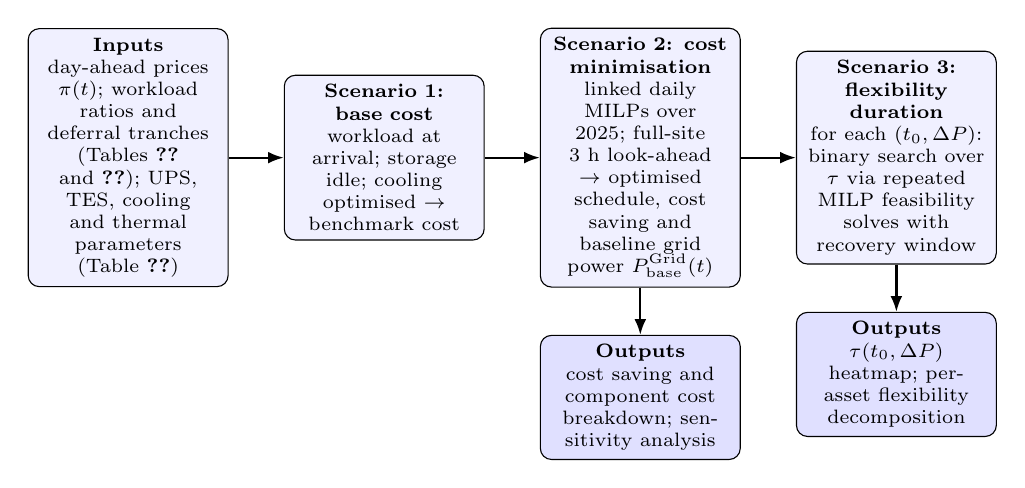
\begin{tikzpicture}[
node distance=6mm and 7mm,
box/.style={draw, rounded corners, align=center, font=\scriptsize, minimum height=9mm, text width=0.19\textwidth, fill=blue!6},
outbox/.style={draw, rounded corners, align=center, font=\scriptsize, minimum height=9mm, text width=0.19\textwidth, fill=blue!12},
arr/.style={-{Latex[length=2mm]}, thick}
]
\node[box] (inputs) {\textbf{Inputs}\\ day-ahead prices $\pi(t)$; workload ratios and deferral tranches (Tables~\ref{tab:workload-rates} and \ref{tab:shiftable}); UPS, TES, cooling and thermal parameters (Table~\ref{tb:nomenclature})};
\node[box, right=of inputs] (s1) {\textbf{Scenario 1: base cost}\\ workload at arrival; storage idle; cooling optimised $\rightarrow$ benchmark cost};
\node[box, right=of s1] (s2) {\textbf{Scenario 2: cost minimisation}\\ linked daily MILPs over 2025; full-site 3 h look-ahead $\rightarrow$ optimised schedule, cost saving and baseline grid power $P^{\mathrm{Grid}}_{\mathrm{base}}(t)$};
\node[box, right=of s2] (s3) {\textbf{Scenario 3: flexibility duration}\\ for each $(t_0,\Delta P)$: binary search over $\tau$ via repeated MILP feasibility solves with recovery window};
\node[outbox, below=of s3] (out3) {\textbf{Outputs}\\ $\tau(t_0,\Delta P)$ heatmap; per-asset flexibility decomposition};
\node[outbox, below=of s2] (out2) {\textbf{Outputs}\\ cost saving and component cost breakdown; sensitivity analysis};
\draw[arr] (inputs) -- (s1);
\draw[arr] (s1) -- (s2);
\draw[arr] (s2) -- (s3);
\draw[arr] (s2) -- (out2);
\draw[arr] (s3) -- (out3);
\end{tikzpicture}}%
\caption{\rev{Workflow of the three-scenario optimisation and flexibility assessment. Scenario 1 provides the workload-at-arrival cost benchmark, Scenario 2 establishes the cost-optimised baseline, and Scenario 3 identifies certified feasible flexibility durations for each requested start time and power deviation while enforcing recovery.}}
\label{fig:workflow}
\end{figure*}

A hypothetical data centre with 1 MW IT capacity and associated infrastructure is considered. Annual electricity prices are the 2025 Great Britain day-ahead Intermittent Market Reference Prices (IMRP) published by the Low Carbon Contracts Company~\cite{lccc_imrp_actuals}. Each hourly price is applied to four quarter-hour intervals, retaining negative values. Table~\ref{tb:energy_price} gives prices for the selected illustrative day, 22 September 2025; annual costs use all 365 days. The final look-ahead uses actual 1 January 2026 prices rather than repeating an earlier day's prices. All principal parameter values remain detailed in Table~\ref{tb:nomenclature}. The 1 MW value is the IT rating, while the structural grid-import bound is 1,723.095 kW including cooling, UPS charging and auxiliaries. Workload profiles repeat by local clock time, with fixed ambient temperature and COP.

\begin{table*}[!t]
\caption{Day-Ahead Reference Prices on 22 September 2025}
\label{tb:energy_price}
\centering
\resizebox{\textwidth}{!}{%
\small
\begin{tabular}{l|*{24}{c}}
\toprule
\textbf{Hour} & 0 & 1 & 2 & 3 & 4 & 5 & 6 & 7 & 8 & 9 & 10 & 11 & 12 & 13 & 14 & 15 & 16 & 17 & 18 & 19 & 20 & 21 & 22 & 23 \\
\midrule
\textbf{Price (GBP/MWh)} & 60.37 & 58.18 & 55.13 & 53.29 & 54.32 & 68.13 & 94.75 & 105.38 & 103.19 & 87.89 & 79.76 & 71.95 & 69.94 & 65.74 & 71.41 & 73.49 & 81.35 & 100.79 & 125.83 & 124.39 & 110.42 & 88.80 & 83.04 & 82.69 \\
\bottomrule
\end{tabular}
}
\end{table*}

\subsection{Scenario 1: Base Cost Calculation}\label{sec:scenario 1}
This scenario calculates the overall cost with workload executed at arrival and without UPS or TES dispatch, while cooling is cost optimised within the same thermal limits as Scenario 2. The purpose of this scenario is to define a base case that provides a benchmark for measuring the potential savings achieved through demand side flexibility. The total DC electricity cost is defined as:

\begin{flalign}
& \sum_{t \in T}
\bigl(
P^{\mathrm{Grid}}_{\mathrm{IT}}(t)
+ P^{\mathrm{Grid}}_{\mathrm{OD}}
+ P^{\mathrm{Chil}\text{-}\mathrm{CRAC}}(t)
\bigr) \cdot \Delta t \cdot \pi(t)/1000, && \\
%
& \rev{P^{\mathrm{Grid}}_{\mathrm{OD}} = \gamma_{\mathrm{OD}} \cdot \overline P^{\mathrm{legacy}}_{\mathrm{IT+cool}}=0.07\times758.5=53.095\ \mathrm{kW}} &&
\end{flalign}

where $\pi(t)$ is the signed day-ahead reference price at time $(t)$ in GBP/MWh; the factor $1/1000$ converts kW to MW. The expression is settled over each committed day and summed over 2025. The UPS and TES tank are not utilised and so incur no dispatch electricity cost in this scenario. \rev{The auxiliary-device power $P^{\mathrm{Grid}}_{\mathrm{OD}}$ is a fixed overhead assumption rather than an optimisation decision: it was calibrated as a fraction $\gamma_{\mathrm{OD}}=0.07$ (7\%) of an earlier daily base-case IT-plus-cooling mean of 758.5 kW, giving the constant value reported in Table~\ref{tb:nomenclature}, and it is held constant in all scenarios rather than recalculated from annual operation.} Additionally, all IT workload executes at arrival, while temperatures evolve within the same bounds as in the coordinated case. These adaptations isolate the additional benefit of workload shifting and storage coordination beyond cost-optimised cooling.

\subsection{Scenario 2: Cost Minimisation}\label{sec:scenario 2}
This scenario calculates the cost-optimised operating conditions by shifting IT workloads over time, utilising the UPS as an energy storage system (ESS), and leveraging the thermal mass of the DC and TES tank for energy storage. This optimisation is highly dependent on the electricity pricing mechanism. In this study, a set of day-ahead spot electricity prices is utilised\rev{, and the annual price variation is represented directly, while resource sensitivities are evaluated in Section~\ref{sec:sensitivity}}. The objective function is to minimise the DC total electricity cost, as defined in Equation (\ref{eq:cost_minimisation}). This is subject to some additional constraints presented in Equations (\ref{eq:43}-\ref{eq:46}). Equation (\ref{eq:43}) ensures that the power supplied to the IT equipment from the grid and the UPS sums to the optimised IT power demand ($P^{\mathrm{IT}}_{\mathrm{opt}}(t)$), which is defined in Equation (\ref{eq:power_optimised}). \rev{Power from auxiliary devices, $P^{\mathrm{Grid}}_{\mathrm{OD}}$, is kept constant at the value defined in Scenario 1, so it is included in the objective but is not an optimisation decision.} Equation (\ref{eq:46}) enforces the non-negativity of all power variables.

Note that the objective explicitly includes grid withdrawals (e.g. \(P^{\mathrm{Grid}}_{\mathrm{IT}}(t)\)) and charging powers (e.g. \(P^{\mathrm{UPS}}_{\mathrm{ch}}(t)\), \(P^{\mathrm{Chil}\text{-}\mathrm{TES}}(t)\)). UPS discharge \(P^{\mathrm{UPS}}_{\mathrm{disch}}(t)\) therefore does not appear directly in the cost sum; its economic effect is realised implicitly through Equation~(\ref{eq:43}), which reduces \(P^{\mathrm{Grid}}_{\mathrm{IT}}(t)\) when the UPS discharges.

% *** NEW FIX: Put Cost equations (40-42) in a figure* float ***
\begin{figure*}[!t]
% --- REMOVED \centering ---
\normalsize
% --- Switched to 'flalign' ---
\begin{flalign}
% --- Added a second '&' at the end of each line ---
& \min \sum_{t \in T^{\mathrm{ext}}}
\bigl(
P^{\mathrm{Grid}}_{\mathrm{IT}}(t)
+ \rev{P^{\mathrm{Grid}}_{\mathrm{OD}}}
+ P^{\mathrm{UPS}}_{\mathrm{ch}}(t)
+ P^{\mathrm{Chil}\text{-}\mathrm{CRAC}}(t)
+ P^{\mathrm{Chil}\text{-}\mathrm{TES}}(t)
\bigr) \cdot \Delta t \cdot \pi(t)/1000, & \label{eq:cost_minimisation} \\
%
& P^{\mathrm{IT}}_{\mathrm{opt}}(t) = P^{\mathrm{Grid}}_{\mathrm{IT}}(t) + P^{\mathrm{UPS}}_{\mathrm{disch}}(t), \quad \forall t \in T^{\text{ext}} & \label{eq:43} \\
%
& 0 \leq P^{\mathrm{Grid}}_{\mathrm{IT}}(t), \rev{P^{\mathrm{Grid}}_{\mathrm{OD}}}, P^{\mathrm{UPS}}_{\mathrm{ch}}(t), P^{\mathrm{Chil}\text{-}\mathrm{CRAC}}(t), P^{\mathrm{Chil}\text{-}\mathrm{TES}}(t), \quad \forall t \in T^{\text{ext}} & \label{eq:46}
\end{flalign}
\hrulefill
\vspace*{4pt}
\end{figure*}
% *** END NEW FIX ***

\rev{The resulting optimisation problem is a Mixed-Integer Linear Program (MILP), as it includes binary variables for the UPS charging/discharging status and TES operation alongside continuous power, energy, temperature and CPU-utilisation decision variables.} In this scenario, the integrated DC model is used in linked daily MILP optimisations over the full year. To maintain the model's linearity, the non-linear function in Equation~\ref{eq:power_it} is linearized using a piecewise linear approximation. This technique approximates the non-linear curve with a series of connected line segments. The implemented four segments have breakpoints $b_i=(i/4)^{1.5}$, $i=0,\ldots,4$, and use Pyomo's DLOG representation; the maximum approximation error is 6.241 kW (0.624\% of rated IT power). Scenario 1 evaluates the identical interpolation at its fixed utilisation. The model was implemented in Python using the Pyomo modelling library and solved using HiGHS. The retained run record identifies Python 3.12.0, Pyomo 6.10.1 and HiGHS 1.15.1 on Windows 11 with an AMD Ryzen 7 9800X3D. The standard daily time limit is 300 s and requested relative MILP gap 0.1\%; feasible time-limited solutions and diagnostic checks are disclosed in Supplementary Section~S5. These linked solves are not a single globally optimal year-long programme.



\subsubsection{Annual operation and cost accounting}\label{sec:annual-operation}
Scenarios 1 and 2 are evaluated over all 365 local days of 2025. Each solve contains the local-day core $T_d$ and twelve look-ahead intervals, with full workload arrivals, cooling and storage operation throughout. Only core decisions are committed. The next day inherits UPS and TES energy, all four temperatures and each unfinished arrival/tranche pair with its original execution window. Look-ahead controls are reoptimised; their trial execution is not counted as completed work.

For a cohort available in day $d$, its committed residual is
\begin{equation}
A_{t,k,d+1}=A_{t,k,d}-\sum_{s\in T_d\cap W_{t,k}}u(t,k,s)\Delta t,
\label{eq:cohort-handoff}
\end{equation}
provided it has arrived before the next core boundary. New look-ahead arrivals are generated afresh when their arrival day is processed. Physical time follows a continuous UTC timeline; local-day and workload labels use Europe/London. Normal days have 96 committed intervals, with 92 and 100 on daylight-saving transitions. The resulting year contains 35,040 quarter-hours.

Annual settlement counts each committed interval once:
\begin{equation}
C^{(i)}_{\mathrm{year}}=\sum_{d=1}^{365}\sum_{t\in T_d}P^{\mathrm{Grid},(i)}(t)\pi(t)\Delta t/1000,
\label{eq:annual-cost}
\end{equation}
where $i=1,2$. The percentage saving is $100(C^{(1)}_{\mathrm{year}}-C^{(2)}_{\mathrm{year}})/C^{(1)}_{\mathrm{year}}$. Overlapping look-ahead costs are excluded until their intervals become committed. Actual prices for the first three hours of 1 January 2026 supply the final continuation; these intervals are outside 2025 settlement. No terminal storage credit is imposed. Supplementary Section~S2 details the procedure and year-end workload treatment, and Section~S5 records existing terminal and solver checks.

This retrospective annual assessment uses known inputs within each daily horizon. It avoids extrapolating a single day's savings, while leaving forecast uncertainty, network tariffs, battery degradation and flexibility-service revenues outside the objective. The event assessment uses the resulting operating trajectory; the rolling procedure provides temporal coverage and continuity rather than the paper's principal methodological contribution.


\subsection{Scenario 3: Flexibility Duration Calculation}\label{sec:scenario 3}
The third scenario evaluates the data centre's capacity to provide flexibility in response to a direct grid signal. This approach models a realistic situation where the grid operator requests a specific magnitude of power change for a certain duration, for example during planned balancing events or unforeseen emergencies. The optimised baseline from Scenario 2 is taken and from it a certified feasible duration for which the DC can sustain specified levels of flexibility magnitude is determined. This is calculated at any given time slot over the 24-hour period. Here, flexibility magnitude, $\Delta P$ (kW), is defined as the power deviation from the optimised baseline; with upward flexibility (load reduction) represented by negative magnitudes and downward flexibility (load increase) by positive magnitudes. For each combination of start time $t_0$ and requested flexibility magnitude $\Delta P$, a continuous period $\tau$ is identified over which the system can track a correspondingly modified grid-power trajectory while maintaining operational feasibility and respecting all physical and thermal constraints. This temporal measure of flexibility provides a key input for assessing the DC's potential participation in demand-response schemes and ancillary-services markets by quantifying its ability to meet specific grid needs.

The flexibility analysis takes the optimised baseline from Scenario \ref{sec:scenario 2} as the reference trajectory and fixes the initial states at the chosen start time $t_0$. Each IT job may already have been shifted by a variable amount, so its remaining flexibility is its original execution window less the time already elapsed. The original four classes are retained, but unfinished work is tracked for each arrival/tranche pair rather than aggregated into new delay classes. Equations~\ref{eq:k_def} and \ref{eq:Dk_def} express the remaining eligible execution window. This prevents a job that has already been deferred from receiving a fresh full deferral allowance.

Another constraint added to the formulation described in Section~\ref{sec: methodology} is the core requirement to deviate the power drawn from the grid, relative to the Scenario 2 baseline, at the requested level over the chosen window. Denoting the baseline grid power draw as $P^{\mathrm{Grid}}_{\mathrm{base}}(t)$ and the new grid power draw as $P^{\mathrm{Grid}}(t)$, the flexibility constraint is given in (\ref{eq:flex_constraint}).

\begin{align}
& K=\{1,2,3,4\},\quad (t,k)\in\mathcal A_{t_0} \label{eq:k_def} \\
& W^{\mathrm{event}}_{t,k}=\{s:\max(t,t_0)\leq s\leq t+D_k\}\cap T^{\mathrm{event}} \label{eq:Dk_def} \\
& \left|P^{\mathrm{Grid}}(t)-P^{\mathrm{Grid}}_{\mathrm{base}}(t)-\Delta P\right|\leq P_{\mathrm{tol}},\quad t_0\leq t<t_0+\tau. \label{eq:flex_constraint}
\end{align}

For each start time $t_0$ and flexibility magnitude $\Delta P$, the feasibility of providing the given $\Delta P$ is tested over a series of durations. \rev{The optimisation described in Scenario 2 is run for each duration over the event and a further twelve-slot (three-hour) recovery window. The flexibility constraint in Equation~\ref{eq:flex_constraint} applies only during service delivery. During recovery, all physical, thermal, storage and workload constraints continue to apply but the grid-power deviation is no longer enforced.} At recovery boundary $H=t_0+\tau+3$ h, UPS and TES energy must be at least their undisturbed Scenario 2 values, each of the four temperatures must be within $0.05^\circ$C of its corresponding value, and every cohort's unfinished work must be no greater than its undisturbed residual plus $10^{-7}$ CPU-hours. Recovery work remains schedulable within its original execution windows; it is not all reclassified as inflexible. These comparative conditions prevent additional depletion or unfinished work from being left beyond recovery.

If an audited feasible solution is found for a given duration $\tau$, the DC can provide that level of flexibility for the given duration. The same feasibility test is then repeated for a longer duration; shorter candidates are explored after unsuccessful trials. The duration is modified using a logarithmic search, with an adjacent-duration check. Candidate durations are multiples of 15 minutes and capped at twelve hours or the remaining local day. An unresolved solve is not proof of infeasibility. Moreover, changing $\tau$ changes the recovery boundary and its reference states, so adjacent checks do not prove that all longer durations are infeasible. The results are therefore certified feasible durations found by the search, with cap-reaching and unresolved-next-step cases identified separately. Supplementary Section~S3 gives the full procedure and status conventions.

The assessment uses 22 September 2025, selected by the smallest standardised distance to twelve annual daily price, demand, cost, utilisation and opening-state features among eligible 96-slot days. Starts are sampled hourly; requests are $-100$ to $-500$ kW in 50 kW steps and $+25$, $+50$ and $+75$ kW, giving 288 combinations. Each event inherits the actual coordinated state and cohort ledger, without preconditioning. All scenarios retain the same $18$--$23^\circ$C cold-aisle bounds. The selected day illustrates state-dependent capability; it does not measure annual service availability.

\subsection{\rev{Sensitivity Analysis Design}}\label{sec:sensitivity-design}
\rev{To assess the dependence of the cost-optimisation results on resource assumptions, a one-at-a-time (OAT) sensitivity analysis is performed around the base case, covering the IT load flexibility ratio and equipment sizing. The flexible workload share is scaled by moving load between the flexible and inflexible pools while preserving the total CPU demand in every time slot, so that the flexibility share is isolated from the demand level; at high multipliers the share saturates in slots that are already almost fully flexible. The TES and UPS energy capacities are scaled while keeping their charge/discharge power limits unchanged, isolating the sizing of the energy buffers. Multipliers are $0.5$, $0.75$, $1.25$ and $1.5$, with the shared central case completing each curve. All cases cover 365 days and use the same workload-at-arrival annual comparator. Storage initial energy fractions and the 50\% UPS reserve fraction are preserved as capacities change. Annual observed prices replace the earlier separate price-volatility perturbation. The results are presented in Section~\ref{sec:sensitivity}.} Additional UPS savings are compared with annualised incremental investment, using a capital recovery factor; the main results give a compact screen and Supplementary Section~S6 states its assumptions.

\subsection{Scenario 1 and 2: Operating Profiles}
Figure \ref{fig:stacked_images} juxtaposes power and workload profiles in subfigures (a) and (b) to highlight optimisation impacts on the selected day, 22 September 2025. Subfigure (a) shows the base and optimised grid power of the DC and the day-ahead electricity reference price. Subfigure (b) shows the combined CPU utilisation of all the servers in the DC over time. The dashed reference shows the CPU utilisation before IT workload shifting has taken place. The stacked areas show CPU utilisation after IT workload shifting. The grey area shows the inflexible workload which cannot be shifted, and the blue area shows flexible workload as executed; the green line gives their total. The opening physical states and unfinished workloads are inherited from the preceding day, rather than reset for this illustration.

Subfigure (a) shows how the optimisation algorithm shifts power consumption away from some higher-price periods. Subfigure (b) shows how the IT workload is rescheduled within its permitted execution windows. The difference between total arrival and execution shows when work is deferred and subsequently processed. The y-axis shows the CPU utilisation of all the servers in the data centre, which has a maximum value of 1. The shifting shown in Figure \ref{fig:stacked_images}(b) changes both IT electricity demand and the heat that must be removed by cooling.




The amount of load shifted to later slots illustrates the optimiser using the available execution windows to avoid higher energy prices. IT workload deferral during a period of rising prices is useful when prices fall within the remaining execution window or when other facility constraints favour the change. The daily pattern also depends on storage states and unfinished work inherited from earlier intervals. Thus a price profile alone does not explain every execution decision, and the annual cost saving cannot be inferred from this selected day.

\begin{figure}[!t]
 \centering
 \subfloat[]{
\includegraphics[width=\columnwidth]{images/Figure_4a.png}%
 \label{fig:power_chart}}
 \vspace{2mm} 
 \subfloat[]{
\includegraphics[width=\columnwidth]{images/Figure_4b.png}%
 \label{fig:it_load_chart}}
 \caption{(a) Grid power and reference prices on 22 September 2025. (b) The corresponding IT workload arrival and execution profiles. Scenario 2 supplies the undisturbed trajectory for the event assessment.}
 \label{fig:stacked_images}
\end{figure}


Figure~\ref{fig:power_resource_stack_chart} provides a detailed decomposition of the data centre's power consumption and resource dispatch strategy under the cost-minimisation objective of Scenario 2. The chart visualises the co-optimised management of various electrical loads and energy storage assets over the 24 hour period. The positive stacked areas represent the components of power drawn from the grid, including IT, CRAC, and charging power for the energy storage systems. The negative stacked areas indicate UPS discharge supplying IT demand. TES discharge reduces the direct chiller electricity needed for cooling; it is not a separate electrical injection. The dotted black line represents the base DC power demand before optimisation, serving as a baseline to illustrate the impact of the flexibility measures.
\begin{figure}[!t]
 \centering
 
\includegraphics[width=\columnwidth]{images/Figure_5.png}
 \caption{Optimised DC Component Power Consumption}
 \label{fig:power_resource_stack_chart}
\end{figure}

When electricity prices are favourable, the optimisation algorithm can draw more power from the grid than required in the base case. This surplus energy can charge the TES tank, effectively storing cooling produced with cheaper electricity, or charge the UPS. It can also be used to process eligible IT workloads, with a consequent change in CRAC power consumption. Conversely, grid power can be reduced by dispatching the TES tank and UPS and by shifting IT workload as shown in Figure~\ref{fig:stacked_images}(b). These decisions establish the operating baseline from which the following flexibility requests are assessed; their annual economic effect is reported after the physical flexibility results.

\subsection{Scenario 3 Results}
Scenario 3 proposes a comprehensive test to identify certified feasible flexibility durations for a set of flexibility magnitudes and start times. The resulting data is three-dimensional and can be effectively visualised as a heatmap. This heatmap is shown in Figure \ref{fig:flex_duration_hourly_heatmap}, with $\tau$ represented by the colour and ($t_0$, $\Delta P$) shown on the (x, y) axes. \rev{Each cell corresponds to one evaluated $(t_0, \Delta P)$ pair, with the printed value giving a certified feasible duration $\tau$ in hours. The underlying model operates at a 15-minute resolution; the assessed start times are sampled hourly across the operating day. The top three rows (positive $\Delta P$) correspond to downward flexibility and the remaining rows (negative $\Delta P$) to upward flexibility.}
\begin{figure*}[!t]
 \centering
 
\includegraphics[width=\textwidth]{images/Figure_6.png}
 \caption{\rev{Flexibility provision magnitude and duration. Cell values are certified feasible durations $\tau$ in hours for each start time $t_0$ (x-axis) and requested power deviation $\Delta P$ (y-axis). Positive $\Delta P$ (top three rows) denotes downward flexibility (load increase) and negative $\Delta P$ denotes upward flexibility (load reduction). A plus sign marks an unresolved next 15-minute trial. Blank cells have no positive duration certified by the search; twelve-hour and local-day-end values are assessment-capped.}}
 \label{fig:flex_duration_hourly_heatmap}
\end{figure*}

Figure~\ref{fig:flex_duration_hourly_heatmap} illustrates significant variations in flexibility duration $\tau$ with start time $t_0$ and deviation $\Delta P$. A 100 kW upward request can be sustained for 1.25 h from 06:00 and 6 h from noon; a 150 kW reduction also lasts 6 h from noon. A 25 kW downward request reaches the twelve-hour assessment cap at 03:00, 10:00, 11:00 and 12:00. These changes reflect the specific baseline from which flexibility is provided: storage energy, unfinished work and thermal conditions differ between starts despite unchanged installed capacities.

Another clear observation is that larger requested magnitudes generally have shorter certified durations, although plateaus occur. Larger deviations require more flexibility per time slot, while recovery also constrains the response. The positive and negative request ranges differ in magnitude, so their durations do not isolate direction from request size. Late-day durations are additionally limited by the end of the selected day. Thirteen cells have an unresolved next trial: for example, a 25 kW increase at 06:00 is feasible for at least 11.25 h and a 50 kW increase for at least 8.75 h. A timeout does not establish an infeasible longer response, and even an adjacent infeasible duration does not prove global maximality under the moving recovery reference.

Each of the elements in Figure \ref{fig:flex_duration_hourly_heatmap} can be decomposed and visualised as a stacked bar chart. A range of these stacked bar charts are shown in Figures \ref{fig:stacked_barcharts_neg} and \ref{fig:stacked_barcharts_pos}. \rev{The plotted decomposition is an accepted feasible dispatch returned by the MILP for the given start time, flexibility magnitude and certified duration. The event-plus-recovery electricity-cost objective selects among feasible dispatches, subject to the recorded solver gap; the component contributions shown should therefore be interpreted as one economically preferred realisation of the flexibility provision rather than a unique physical decomposition.} In these plots, the duration is shown on the x-axis and the flexibility magnitude on the y-axis. Each stacked bar consists of the different sources of flexibility in the DC, illustrating how much flexibility is being provided by each DC asset throughout the flexibility provision. The dashed line shows the requested cumulative flexibility during the event. The target is released during the post-event region; recovery is checked through the terminal conditions rather than fully displayed in each panel. Notably, in a considerable number of time slots, certain DC assets change their power consumption in the opposite direction to what is required. The other DC assets compensate by adjusting their power consumption to a greater extent, ensuring that the desired net flexibility magnitude is achieved. This is visible in the charts, where the stacked bars include both negative and positive components. This effect clearly illustrates the DC assets working in conjunction to achieve the desired net effect in the data centre.

\begin{figure}[!t]
 \centering
 
\includegraphics[width=\columnwidth]{images/Figure_7.png}
 \caption{\rev{DC component contributions to upward flexibility (negative $\Delta P$). The four panels are arranged in a 2-by-2 grid: rows correspond to the requested flexibility magnitudes ($-100$ and $-200$ kW, top to bottom) and columns to the start times (06:00, left; 15:00, right). Colours show the flexibility contribution of each DC asset.}}
 \label{fig:stacked_barcharts_neg}
\end{figure}

\rev{Figure \ref{fig:stacked_barcharts_neg} presents the upward flexibility (negative $\Delta P$) results as four stacked bar charts arranged into a 2-by-2 grid, in which the rows correspond to the requested flexibility magnitudes ($-100$ and $-200$ kW) and the columns to the start times (06:00 and 15:00). The colours show how much flexibility each DC asset is providing.} Figure \ref{fig:stacked_barcharts_neg} shows that $\tau$ depends strongly on $\Delta P$ and $t_0$. It is intuitive that the larger the flexibility magnitude the shorter the duration it can be provided for. $t_0$ has a large impact on duration due to the specific baseline from which the flexibility is being provided. The left-hand side of Figure~\ref{fig:stacked_barcharts_neg} shows the morning response: the selected 100 and 200 kW reductions at 06:00 are provided entirely by additional UPS discharge for 1.25 h. At 15:00, both reductions last 3 h and are provided mainly by IT workload deferral and reduced direct cooling. Additionally, cooling power reduction can take place when there is IT workload shifting as less heat is generated by the servers. TES is full and idle in the undisturbed trajectory at that afternoon start, so there is no TES charging to curtail. The 200 kW case uses IT and cooling alone, while the 100 kW case includes a single 37 kW UPS-discharge interval. Thus the participating resources change with the operating state; installed capacity alone does not determine which asset provides the response.

\begin{figure}[!t]
 \centering
 
\includegraphics[width=\columnwidth]{images/Figure_8.png}
 \caption{\rev{DC component contributions to downward flexibility (positive $\Delta P$). Rows correspond to the requested flexibility magnitudes ($+25$ and $+75$ kW, top to bottom) and columns to the start times (00:00, left; 06:00, right). Colours show the flexibility contribution of each DC asset.}}
 \label{fig:stacked_barcharts_pos}
\end{figure}

\rev{Figure \ref{fig:stacked_barcharts_pos} presents the downward flexibility (positive $\Delta P$) results, with magnitudes of $+25$ and $+75$ kW and start times 00:00 and 06:00.} As  with the upward flexibility charts, $\tau$ depends strongly on  $\Delta P$ and $t_0$. The IT workload, CRAC, TES charging and UPS net exchange contribute through changes that may reinforce or oppose one another. Eligible work can be executed earlier than in Scenario 2, provided that it has already arrived. At 06:00, the 25 kW increase lasts at least 11.25 h and the 75 kW increase 7.75 h. One approach could be to include a `charge up' time before the flexibility window where earlier time slots could reschedule their workload to later time slots in the flexibility window. This is akin to the recovery time slot implemented after the flexibility provision. Another notable result is the large positive and negative magnitudes exhibited by different DC assets within the same timeslot. As mentioned previously, these assets provide opposing flexibility responses that cancel each other out to achieve the desired effect. This allows one asset to provide flexibility while the other ``recharges'' its flexibility potential, thereby demonstrating the value of an integrated DC model.

\subsection{Scenario 1 and 2: Annual Electricity Costs}
\rev{The total annual base and optimised costs are GBP~550,503.59 and GBP~522,702.95, respectively, representing a GBP~27,800.64 cost saving. This demonstrates that, with an appropriate management algorithm, the modelled data centre flexibility assets can be used for electricity-cost minimisation, yielding savings of 5.05\%. The calculation includes conversion losses and preserves computational work, but excludes degradation, additional operating costs and service revenues.}

Annual grid electricity increases from 6.718 to 6.794 GWh (approximately 1.13\%), and peak import increases from 974.9 to 1,681.9 kW. Lower expenditure therefore does not imply lower electricity use or lower network peak demand. The valuation includes all observed 2025 prices, including 672 negative-price quarter-hours, whereas the selected physical-assessment day has none. It is a reference-price electricity-cost comparison rather than a complete site bill or market-revenue calculation.

\rev{Table~\ref{tab:cost-breakdown} decomposes the total annual electricity cost of both scenarios by component. In the base case, IT load dominates the cost (74\% of the total), followed by cooling (19\%) and the constant auxiliary overhead (7\%). Over 2025, the optimisation reduces the IT electricity-cost term by GBP~15,243.51 and direct CRAC cooling by GBP~14,084.33. TES charging adds GBP~6,903.30, while net UPS exchange reduces expenditure by GBP~5,376.10; auxiliary expenditure is unchanged. These are signed accounting terms in the integrated schedule, not independent asset profits: TES benefits appear partly through reduced direct chiller demand, and the UPS term is charging minus discharging valued at interval prices. The net effect is the overall saving of GBP~27,800.64 (5.05\%).}

\begin{table*}[htbp]
\centering\small
\caption{Annual signed electricity-cost composition (GBP). Changes are coordinated minus reference; displayed values are rounded.}\label{tab:cost-breakdown}
\begin{tabular}{@{}lrrr@{}}\toprule
Component & Scenario 1 & Scenario 2 & Change \\\midrule
IT electrical demand & 407,653 & 392,409 & -15,244 \\
CRAC chiller & 105,337 & 91,252 & -14,084 \\
TES charging chiller & 0 & 6,903 & +6,903 \\
UPS net grid effect & 0 & -5,376 & -5,376 \\
Auxiliary overhead & 37,514 & 37,514 & +0 \\
Total settlement cost & 550,504 & 522,703 & -27,801 \\
\bottomrule\end{tabular}
\end{table*}

\subsection{\rev{Sensitivity Analysis}}\label{sec:sensitivity}
\rev{Figure~\ref{fig:sensitivity_tornado} summarises the OAT sensitivity analysis described in Section~\ref{sec:sensitivity-design} using the full-year electricity-cost saving. The base case yields a 5.05\% saving; each curve shows the response when the corresponding resource parameter is varied between $0.5\times$ and $1.5\times$ its base value. All intermediate points are completed annual runs.}

\rev{The cost saving is most sensitive to the flexible workload share among the resource variations tested: halving the share reduces the saving to 3.522\%, while increasing it by $1.5\times$ raises the saving to 6.257\%. At high multipliers the realised share saturates in slots where all arriving work is already flexible. Varying UPS energy capacity between $0.5\times$ and $1.5\times$ changes the saving between 4.565\% and 5.501\%, while varying TES capacity over the same range changes it between 4.800\% and 5.167\%. Storage power ratings remain fixed, so larger energy buffers do not remove charge/discharge or chiller limits. These results quantify dependence on the adopted workload and equipment assumptions rather than establishing robustness to all uncertainties or comparing resources at equal investment cost. The full annual results and solver exceptions are provided in Supplementary Sections~S4--S5.}

\begin{figure}[!t]
 \centering
 
\includegraphics[width=\columnwidth]{images/Figure_9.png}
 \caption{\rev{Change in annual saving, in percentage points from the central case, for one-at-a-time resource variations. Panel (a) uses the realised flexible share after clipping. Note the different vertical scales.}}
 \label{fig:sensitivity_tornado}
\end{figure}

\subsubsection{Incremental value of larger UPS batteries}
The UPS sensitivity addresses whether additional energy capacity could be justified partly by its flexibility value. Increasing the central 600 kWh capacity to 750 and 900 kWh produces additional annual electricity-cost savings of GBP~1,292.28 and GBP~2,481.41, respectively. With the reserve fraction fixed at 50\%, the additions of 150 and 300 nameplate kWh increase the operational energy window by 75 and 150 kWh. Power ratings remain unchanged.

For a constant annual incremental saving $\Delta S$, additional annual non-electricity cost $O$, real discount rate $r$ and life $n$, the break-even incremental investment is
\begin{equation}
I_{\mathrm{BE}}=\frac{\Delta S-O}{\mathrm{CRF}(r,n)},\qquad
\mathrm{CRF}(r,n)=\frac{r(1+r)^n}{(1+r)^n-1}.
\label{eq:ups-investment}
\end{equation}
The capital recovery factor annualises initial expenditure~\cite{sam_crf}. At an illustrative 8\% real rate over ten years, with $O=0$, the additional savings support investments of approximately GBP~8,671 and GBP~16,650, or GBP~57.81 and GBP~55.50 per added nameplate kWh. These are expenditure thresholds, not installed battery prices or an unconditional case for enlargement. Installation, degradation, O\&M and replacement costs would need to be covered, and the retained single-year savings are not demonstrated lifetime cash flows: initial and terminal energy differ between capacities. Supplementary Section~S6 gives the assumptions and alternative rate/life combinations. No revenue for the physical flexibility events is added to these electricity-cost savings.


\subsection{\rev{Value of Integrated Co-optimisation}}\label{sec:integration-value}
\rev{The results allow the central question of what the integrated model reveals that separate, asset-level models would miss to be answered directly. First, the IT--cooling coupling: upward flexibility obtained by deferring IT workload produces a secondary reduction in cooling power because less heat is generated. A stand-alone IT flexibility model would omit the associated cooling-power change, while a stand-alone cooling model with fixed IT demand would not represent the deferred heat load. Second, the change in resource participation visible in Figure~\ref{fig:stacked_barcharts_neg}: morning reductions rely on UPS discharge, whereas afternoon reductions rely mainly on IT deferral and cooling. This temporal coordination is only visible in a model that schedules both assets against a common grid-power trajectory. Third, the TES buffering role: changes in direct CRAC cooling and TES charging interact with the other resources, allowing opposing responses in which one asset ``recharges'' its flexibility potential while others over-deliver, as observed in Figures~\ref{fig:stacked_barcharts_neg} and \ref{fig:stacked_barcharts_pos}. These cross-asset interactions explain why the feasible duration envelope depends so strongly on the baseline operating state, and why a duration-aware, whole-facility formulation is required to characterise feasible grid-facing responses. These dispatch mechanisms do not quantify an integration premium over separately optimised subsystems, which would require an explicit comparator.}

\rev{Finally, the scope of the grid interpretation should be noted. The model characterises the flexibility that the data centre can offer at its grid connection point; assessing the impact of the resulting load profile on upstream network stability or hosting capacity would require network topology, voltage and thermal limits, and the concurrent behaviour of other loads. The outputs of this work are therefore best interpreted as candidate flexibility offers to be evaluated within a system- or network-level study.}

The workload split is context-dependent: applications, customer requirements, incentives and SLAs determine what may be shifted. The repeated daily workload, fixed ambient temperature and COP exclude seasonal and weekly facility changes. GPU power management, task dependencies and other forms of computational flexibility are outside the aggregate CPU-hour representation. The representative-day envelope does not establish annual availability, response speed below the quarter-hour resolution, or eligibility for a particular market product.

\section{Conclusion}

This paper presents an integrated, whole-facility framework that allows a DC to act as a flexible power consumer with quantifiable flexibility provision. By co-optimising IT workload scheduling, UPS-ESS dispatch, and thermodynamic cooling with thermal energy storage, a cost-minimising operating baseline was established through linked daily optimisation over 2025, achieving a \rev{5.05\% reduction in annual electricity costs. A sensitivity analysis showed that the flexible workload share has the greatest effect among the tested resource variations, followed by UPS and TES energy capacity. Increasing UPS capacity from 600 to 900 kWh adds approximately GBP~2,481/year in savings, supporting a conditional incremental investment screen.} Building on this baseline, our core contribution is a duration-aware flexibility assessment that, for any start time ($t_0$) and requested power deviation ($\Delta P$), identifies certified feasible durations ($\tau$) of flexibility provision while enforcing operational constraints and the specified comparative recovery conditions. The resulting flexibility duration envelope reveals a strong temporal structure and a notable asymmetry. Upward flexibility (load reduction) is driven by deferring IT workload, allowing for a reduction in cooling power. At other start times, UPS discharge supplies the reduction without changing IT demand; TES and cooling participate according to the inherited state. In contrast, downward flexibility (load increase) combines changes in IT execution, cooling and storage, including earlier execution of work already available to process. This framework successfully quantifies power deviations and feasible durations under stated recovery rules, turning abstract potential into capabilities that can be assessed against market-specific requirements. Figure \ref{fig:flex_duration_hourly_heatmap} provides a comprehensive set of results for the flexibility potential, detailing how the duration of flexibility provision changes depending on the magnitude required and specific start time. Results show a significant change in flexibility potential, with $100$ kW of upward flexibility possible for $6$ hours at noon and $1.25$ hours at $06$:$00$. This change reflects the varying operating conditions of the baseline from which flexibility is being provided. \rev{The trade-off between magnitude and duration is equally clear: a $25$ kW increase reaches the twelve-hour assessment cap at several start times, while larger tested requests generally have shorter certified durations. Cap-reaching results and unresolved adjacent trials are not intrinsic maximum-duration estimates. Interpreted per MW of IT capacity, these results indicate that the modelled data centre can sustain power deviations of the order of $10\%$ of its IT capacity for multiple hours, with the feasible envelope determined by the start time and the requested magnitude.}

Promising future work includes incorporating explicit revenue stacking, exploring a ``pre-conditioning'' window to assess additional IT participation in downward events, and aggregating facilities to a portfolio scale. Ultimately, the methodology presented offers a practical pathway for integrating data centres into power system operations, characterising candidate grid responses alongside annual electricity-cost savings. Those savings do not imply lower energy consumption or peak import, and service revenues remain outside the present valuation.

% -------- Bibliography --------
% Ensure you have a 'references.bib' file in your project
\bibliographystyle{IEEEtran}
\bibliography{references}

% --- Acknowledgements Section ---
\section*{Acknowledgements}

This work was supported by the Engineering and Physical Sciences Research Council (EPSRC) and the Economic and Social Research Council (ESRC) through funding provided to the Energy Demand Research Centre (grant number EP/Y010078/1).

% --- CRediT Statement Section ---
% Using \noindent and \textbf to format the list clearly.
% The \medskip adds a small vertical space between entries.
\section*{CRediT Authorship Contribution Statement}

\noindent \textbf{James Day:} Writing – original draft, Investigation, Methodology, Conceptualization.

\medskip
\noindent \textbf{Mehmet Türker TAKCI:} Writing – original draft, Investigation, Methodology, Conceptualization.


\medskip
\noindent \textbf{Meysam Qadrdan:} Review \& editing, Supervision, Conceptualization.



\end{document}